% ------------------------------------------------------------------------
%
% ----------------------      Thesis.tex       ---------------------------
%
% ------------------------------------------------------------------------
% ------------------------------------------------------------------------
% ------------------------------------------------------------------------
% Versi�n de plantilla, para realizaci�n de informes de trabajo de grado,
% tomada del ejemplo sugerido en WinEdt 5.3, y modificada para uso de la
% Universidad Nacional de Colombia - Sede Manizales, en agosto de 2003, y
% de la Universidad Industrial de Santander en octubre de 2014.
% ------------------------------------------------------------------------
% ------------------------------------------------------------------------
% ------------------------------------------------------------------------
%
% ------------------------------------------------------------------------

\documentclass[letter,oneside,11pt,spanish]{report}          % Encabezados

\usepackage[spanish,es-nodecimaldot]{babel} % Reconocimiento para letras {\~n} y tildes
\usepackage[ansinew]{inputenc}
\usepackage{graphicx,epstopdf}

\DeclareGraphicsExtensions{.pdf,.png,.jpg,.eps}
\usepackage{xthesis}                    % Paquete de plantilla predise{\~n}ada
\usepackage{epsfig}
\usepackage{amsmath,amssymb,amsfonts}          % Soporte matem�tico
\usepackage{hyperref}                          % Hiperv�nculos y bookmarks
\usepackage{subfigure}                    % Soporte para m�ltiples figuras
\usepackage{booktabs}
\usepackage{xcolor}
\usepackage{psfrag}
\usepackage{url}

% ------------------------------------------------------------------------
% ------------------------------------------------------------------------
\usepackage{amsthm}
\newtheorem{teo}{Teorema}[section]
\newtheorem{mydef}{Definici�n}[section]

\usepackage{caption}
\captionsetup[table]{skip=10pt}

\newlength{\defbaselineskip}
\setlength{\defbaselineskip}{\baselineskip}
\newcommand{\setlinespacing}[1]%
           {\setlength{\baselineskip}{#1 \defbaselineskip}}
\newcommand{\doublespacing}{\setlength{\baselineskip}%
                           {2.0 \defbaselineskip}}
\newcommand{\singlespacing}{\setlength{\baselineskip}{\defbaselineskip}}
% ------------------------------------------------------------------------
% ------------------------------------------------------------------------
% ------------------------------------------------------------------------
\begin{document}                                     % Inicio de documento

% ------------------------------------------------------------------------
% ------------------------------------------------------------------------
% ------------------------------------------------------------------------

% Definici�n sil�bica de palabras

\hyphenation{pro-por-cio-nal}


% ------------------------------------------------------------------------

% Renombramiento para t�tulos en ingl�s

\renewcommand\chaptername    {Cap�tulo}
\renewcommand\listfigurename {Lista de Figuras}
\renewcommand\listtablename  {Lista de Tablas}
\renewcommand\bibname        {Bibliograf�a}
\renewcommand\contentsname   {Tabla de Contenido}
\renewcommand\tablename      {Tabla}
\renewcommand\appendixname   {Anexo}
% ------------------------------------------------------------------------
% Definici�n para elementos de contenido previo a cuerpo del trabajo
% ------------------------------------------------------------------------
% ------------------------------------------------------------------------
% ------------------------------------------------------------------------
% ------------------------------------------------------------------------
%    Definici�n para elementos de contenido previo a cuerpo del trabajo
% ------------------------------------------------------------------------
% ------------------------------------------------------------------------
% ------------------------------------------------------------------------

% ------------------------------------------------------------------------
%                                 Cubierta
% ------------------------------------------------------------------------

\thispagestyle{empty}

\begin{center}

\Large{\textbf{DISE�O E IMPLEMENTACI�N DEL SISTEMA DE PROPULSI�N PARA UN PROTOTIPO PRIMITIVO DE VEH�CULO EL�CTRICO PARA LA E3T-UIS} \vspace{6cm}}

\large{Daniel Eduardo Lizarazo Rosas}\\
\large{Jos� David Angarita Pertuz}\\
\vspace{7.5cm}

\large\textbf{Universidad Industrial de Santander}\\
\textbf{Escuela de Ingenier�as}\\
\textbf{El�ctrica, Electr�nica y de Telecomunicaciones}\\
\textbf{Bucaramanga}\\
\textbf{2021}\\

\end{center}

% ------------------------------------------------------------------------
%                                 Portada
% ------------------------------------------------------------------------

\newpage
\thispagestyle{empty}

\begin{center}

\Large{\textbf{DISE�O E IMPLEMENTACI�N DEL SISTEMA DE PROPULSI�N PARA UN PROTOTIPO PRIMITIVO DE VEH�CULO EL�CTRICO PARA LA E3T-UIS} \vspace{3cm}}

\large{Daniel Eduardo Lizarazo Rosas}\\
\large{Jos� David Angarita Pertuz}\\
\vspace{2.3cm}

\large{Trabajo de Grado para optar al t�tulo de\\
Ingeniero Electricista e Ingeniero Electr�nico}\\\vspace{2.5cm}

\large{Director\\
Ricardo Alzate Casta�o, Ph.D.} \vspace{3.0cm}


\large\textbf{Universidad Industrial de Santander}\\
\textbf{Escuela de Ingenier�as}\\
\textbf{El�ctrica, Electr�nica y de Telecomunicaciones}\\
\textbf{Bucaramanga}\\
\textbf{2021}\\

\end{center}                                                % Portada
% ------------------------------------------------------------------------
% Dedicatoria
%\dedicate {Dedicatoria ...}
% ------------------------------------------------------------------------
\beforepreface \setcounter{page}{3}
% ------------------------------------------------------------------------
%% ------------------------------------------------------------------------
% ------------------------------------------------------------------------
% ------------------------------------------------------------------------
%                                Resumen
% ------------------------------------------------------------------------
% ------------------------------------------------------------------------
% ------------------------------------------------------------------------
\chapter*{RESUMEN}

\footnotesize{
\begin{description}
  \item[T�TULO:] CONTROL �PTIMO DE MICRORREDES A PARTIR DE UN ENFOQUE JER�RQUICO \footnote{Trabajo de grado}
  \item[AUTOR:] SEBASTI�N BENJUMEA CERPA \footnote{Facultad de Ingenier�as F�sico-Mec�nicas. Escuela de Ingenier�as El�ctrica, Electr�nica y Telecomunicaciones. Director: Ricardo Alzate Casta�o, Doctorado en Ingenier�a Inform�tica y Autom�tica.}
  \item[PALABRAS CLAVE:] CONTROL JER�RQUICO, ENERG�AS RENOVABLES, GESTI�N DE RECURSOS ENERG�TICOS, MICRORREDES EL�CTRICAS.
  \item[DESCRIPCI�N:]\hfill \\ El presente trabajo de grado presenta el dise�o e implementaci�n (a trav�s de simulaci�n) de una estrategia para la gesti�n optimizada de recursos energ�ticos en una microrred DC aislada, que hace uso de fuentes renovables. Inicialmente, el trabajo aborda una revisi�n conceptual acerca del control de circuitos convertidores de potencia del tipo elevador (boost) y se complementa por el problema de reparto de potencias a trav�s de esquemas de control droop. Posteriormente, se establece una estructura jer�rquica para gobernar la asignaci�n de proporciones de generaci�n (despacho) en una microrred, atendiendo a criterios de costo definidos considerando recursos renovables. A partir de ello, se toma como caso de estudio una estaci�n de carga para autom�viles el�ctricos, dimensionada para operar a una carga nominal de 1500 W, y a la cual se aplica la estrategia de control jer�rquico utilizando simulaciones en PSIM. Para obtener la asignaci�n din�mica (gesti�n) de recursos en la microrred se realiz� la codificaci�n del algoritmo de Newton-Raphson, como m�todo de aproximaci�n para determinar la soluci�n �ptima del problema y por ende, la reducci�n del costo de operaci�n de la microrred. Trabajos futuros incluyen la extensi�n de los resultados presentados al caso de sistemas de generaci�n en corriente alterna y la verificaci�n experimental para el algoritmo de gesti�n de recursos propuesto.
\end{description}}\normalsize
% ------------------------------------------------------------------------                                                % Resumen
%% ------------------------------------------------------------------------
% ------------------------------------------------------------------------
% ------------------------------------------------------------------------
%                                Abstract
% ------------------------------------------------------------------------
% ------------------------------------------------------------------------
% ------------------------------------------------------------------------
\chapter*{ABSTRACT}

\footnotesize{
\begin{description}
  \item[TITLE:] OPTIMAL CONTROL OF A MICROGRID FROM A HIERARCHICAL VIEWPOINT\footnote{Bachelor Thesis}
  \item[AUTHOR:] SEBASTI�N BENJUMEA CERPA\footnote{Facultad de Ingenier�as F�sico-Mec�nicas. Escuela de Ingenier�as El�ctrica, Electr�nica y Telecomunicaciones. Director: Ricardo Alzate Casta�o, Doctorado en Ingenier�a Inform�tica y Autom�tica.}
  \item[KEYWORDS:] ELECTRICAL MICROGRID, ENERGY RESOURCE MANAGEMENT, HIERARCHICAL CONTROL, RENEWABLE ENERGY.
  \item[DESCRIPTION:]\hfill \\ In this work, the design and implementation through numerical simulation of an energy management strategy for resources of an isolated DC microgrid employing renewable sources, is performed. First of all, a review about concepts regarding the control of DC electronic power circuits of the boost type and the scheduling of power in generation schemes via the so-called droop control technique, are covered in order to configure a hierarchical structure of power management aiming at implementing economic dispatch of resources attending cost requirements for renewable sources, including as part of a microgrid scheme configured to supply the power demand of a charging station for electric vehicles with a nominal load of 1500 W. Accordingly, numerical simulations in PSIM were performed to verify the hierarchical control scheme achieving dynamical scheduling of generation proportions (power management) by modifying the droop parameter subjected to a cost functional suited for renewable sources. Moreover, the implementation of a numerical Newton-Raphson algorithm was performed in a C-code block of PSIM to approximate the optimal solution, reducing the operation cost of the microgrid. Ongoing work include the extension of presented results to the case of alternating current generation systems and the experimental verification for the dispatch algorithm proposed.
\end{description}}\normalsize
% ------------------------------------------------------------------------ 
% ------------------------------------------------------------------------
%% ------------------------------------------------------------------------
% ------------------------------------------------------------------------
% ------------------------------------------------------------------------
%                             AGRADECIMIENTOS
% ------------------------------------------------------------------------
% ------------------------------------------------------------------------
% ------------------------------------------------------------------------
\chapter*{AGRADECIMIENTOS}

Agradezco a mi familia por el apoyo ec�nomico y moral que tuvieron para conmigo
durante el desarrollo de mi carrera. Tambi�n agradezco a mis amigos y
compa�eros por las vivencias de estos inolvidables a�os de universidad.\\

Un reconocimiento y agradecimiento importante lo realizo a mi director de
trabajo de grado, por dedicar su tiempo, experiencia y conocimiento en la gu�a
de mi proyecto.
% ------------------------------------------------------------------------
\newpage                            % Agradecimientos
% ------------------------------------------------------------------------
\tableofcontents                                      % Tabla de contenido
% ------------------------------------------------------------------------
\listoffigures                                 % Lista de figuras y tablas
%\listoftables
% ------------------------------------------------------------------------
% Contenido del Informe
% ------------------------------------------------------------------------
% Cap�tulos
% ------------------------------------------------------------------------
% ------------------------------------------------------------------------
% ------------------------------------------------------------------------
% ------------------------------------------------------------------------
%                   Secci�n de Introducci�n a la Tesis
% ------------------------------------------------------------------------
% ------------------------------------------------------------------------
% ------------------------------------------------------------------------
\chapter{Introducci�n}

\pagenumbering{arabic}\setcounter{page}{1}\label{intro}
% ------------------------------------------------------------------------
% ------------------------------------------------------------------------
La ``descarbonizaci�n'' de la econom�a ha impulsado a gobiernos de todo el mundo a proponer incentivos para acelerar la transici�n de combustibles f�siles
a energ�as de tipo renovable. En particular, un gran esfuerzo econ�mico y tecnol�gico se viene realizando en a�os recientes para aplicar lo anterior a los medios de transporte, incluyendo excepciones tributarias de importaci�n y circulaci�n, subsidios para compra, fabricaci�n o investigaci�n y beneficios log�sticos como v�as exclusivas, espacios de parqueo especial y descuentos de tarifas, entre otros.\\

Un veh�culo el�ctrico (EV - \emph{electric vehicle} de su sigla en ingl�s) es un veh�culo autom�vil, para transporte de personas o de mercanc�as, propulsado por uno o m�s motores el�ctricos, usando energ�a el�ctrica almacenada normalmente en bater�as recargables. La Fig. \ref{partes_vehiculo_EV} ilustra el esquema general para un EV.\\
% ------------------------------------------------------------------------
\begin{figure}[htbp]
\centering		
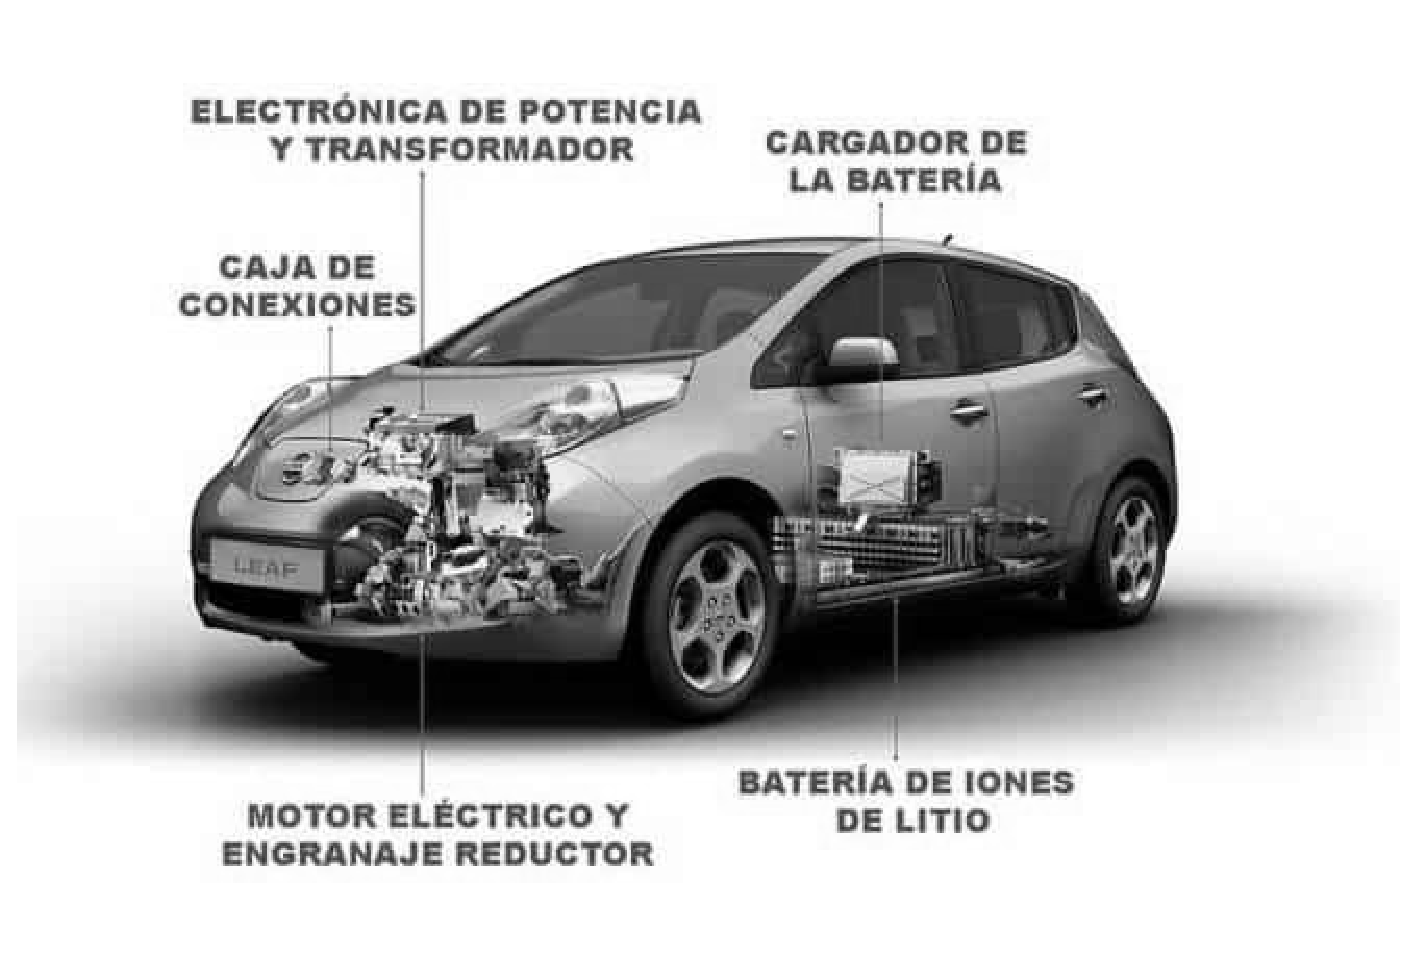
\includegraphics[width=0.5\textwidth]{Figs/Partes-de-un-coche-electrico-gray.eps}
\caption[Partes principales de un EV]{Partes principales de un EV (tomado de \texttt{Wikipedia.org})}\label{partes_vehiculo_EV}
\end{figure}
% ------------------------------------------------------------------------

En el a�o 2010 el gobierno de China puso en marcha un proyecto piloto de incentivos en la compra de autos el�ctricos e h�bridos, complementado en 2012 por una exenci�n de impuestos anuales. A partir de ello, se experiment� un crecimiento en ventas para este tipo de veh�culos en un 328\% para el a�o 2014. No obstante, para reducir las emisiones contaminantes al ambiente se deben complementar estas medidas con cambios en la canasta energ�tica de un pa�s que produce el 75\% de su electricidad a partir de carb�n \cite{masiero2016electric}.\\

Por su parte, Alemania propuso en 2010 la meta de tener circulando un mill�n de EV para 2020, a partir de subsidios en investigaciones para nuevas tecnolog�as y exenciones tributarias anuales de circulaci�n hasta por diez a�os. Sin embargo, a noviembre de 2014 s�lo se hab�a logrado el 25\% de dicha meta, hecho que motiv� un incremento de incentivos para grandes compa��as productoras como Nissan, BMW y Citro�n \cite{loisel2014large}. A pesar de lo anterior, Alemania sigue siendo el pa�s inventor y promotor del motor de combusti�n interna y de la tecnolog�a Di�sel.\\

De otro lado, en los Estados Unidos de Am�rica se plantearon una meta similar en 2011 para tener un mill�n de EV circulando al a�o 2015. Sin embargo, en el a�o 2016 tan s�lo el 50\% de esa meta hab�a sido alcanzada, implicando extender las pol�ticas de incentivos y exenciones para la fabricaci�n y comercializaci�n de partes de EV, cuya venta fue levemente incrementada tras integrarse al paradigma de la red inteligente de distribuci�n energ�tica (\emph{SmartGrid}) \cite{soltani2017analysis}.\\

A nivel latinoamericano, se cuenta con un alto potencial de recursos naturales para la fabricaci�n de bater�as y conductores el�ctricos. Chile ha realizado inversiones importantes en transporte p�blico el�ctrico. M�xico posee plantas de producci�n que se han fijado la meta para 2020 de comenzar a producir EV. Per� ha eliminado las tasas de importaci�n de EV y comienza a dise�ar su plan de movilidad el�ctrica. Paraguay y Brasil cuentan con una amplia cantidad de estaciones instaladas para carga r�pida de EV. Argentina, a pesar de tener una riqueza significativa en litio, no presenta mayores avances en una pol�tica de movilidad el�ctrica debido a los problemas actuales que afronta su econom�a \cite{quiros2019electric}.\\

Por su parte, Colombia en el a�o 2018 fue el primer pa�s de la regi�n en superar los 1000 EV en circulaci�n, aprobando incentivos fiscales para su compra e importaci�n. Asimismo, aprob� una pol�tica nacional de crecimiento verde con la cual se espera tener 600.000 EV (entre veh�culos livianos, taxis, buses, veh�culos gubernamentales y camiones) para 2030. Tambi�n es evidente el aumento de motocicletas el�ctricas circulantes, con m�s de 2000 unidades registradas entre 2011 y 2018. Varias empresas prestadoras de servicio el�ctrico han instalado estaciones de carga r�pida para clientes y usuarios. Desde 2017, las ciudades de Bogot�, Cali y Medell�n han estado probando buses el�ctricos en sus flotas de transporte masivo y han anunciado planes para introducir taxis el�ctricos, algunos en operaci�n desde 2012 \cite{Gobierno_Colombia}. Todo lo anterior est� articulado con la Ley 1964 del 11 junio de 2019 a partir de la cual la Presidencia de la Rep�blica promueve el uso de EV en Colombia \cite{ley_Gobierno_Colombia}.\\

En la Universidad Industrial de Santander, en el a�o de 2010 se desarroll� un concurso de veh�culos de tracci�n humana (VTH) liderado por la Escuela de Ingenier�a Mec�nica. Tambi�n se destaca el trabajo desarrollado por \emph{Ovalle et al.} \cite{coronado2015diseno} quienes realizaron el dise�o y la construcci�n de un prototipo de veh�culo biplaza tipo \emph{Buggy} impulsado a trav�s de un motor de combusti�n interna. Otro aporte interesante fue realizado por \emph{Cuesta y Callejas} \cite{vagon2019} quienes agregaron propulsi�n el�ctrica (motorizaci�n) a un vag�n para aplicaciones de miner�a. Por su parte, \emph{Castro y Pe�a} desarrollaron un prototipo de transporte unipersonal tipo \emph{Segway} \cite{castro2011diseno}. De manera m�s reciente, \emph{Amaya y Rueda} \cite{amaya&rueda2019} realizaron el modelado de una bicicleta el�ctrica utilizando la aproximaci�n energ�tica macrosc�pica. Otros trabajos como el de \emph{Ardila y Ochoa} \cite{ardila2018ubicacion} se orientan al an�lisis de estaciones de recarga para veh�culos el�ctricos, como eventual perturbaci�n del sistema interconectado nacional.\\

En otras Universidades de Colombia la movilidad el�ctrica presenta como su caso m�s representativo el proyecto \emph{EOLO} desarrollado desde 2015 por la Universidad Minuto de Dios \cite{ariza2019educational}. Adicionalmente, en la Universidad Distrital Francisco Jos� de Caldas se realiz� el dise�o y fabricaci�n de un veh�culo impulsado por energ�a solar \cite{aguillon2012diseno} y en la Universidad Militar Nueva Granada se analiz� un caso similar al anterior, pero con almacenamiento energ�tico \cite{arevalo2014diseno}.\\

Otros desarrollos importantes incluyen el proyecto independiente \emph{ECO-City} que construye EV para comercializaci�n en Colombia (\texttt{http://www.eco-citi.com/auto-electrico/}) y los monoplaza el�ctricos elaborados por los aprendices del Servicio Nacional de Aprendizaje (SENA). A nivel latinoamericano, se destaca la contribuci�n del Instituto Polit�cnico Nacional de M�xico \cite{ramos&soto2013} y en Ecuador el trabajo de la Universidad Polit�cnica Salesiana de Cuenca \cite{aguirre2014diseno}. Finalmente, la Universidad Polit�cnica de Catalu�a en Espa�a tambi�n ha realizado aportes en el tema de dise�o de prototipos de EV tal y como se presenta en \cite{martin2016diseno}.\\

A partir de lo anterior es claro que existen antecedentes de trabajos orientados al desarrollo de veh�culos en la Universidad Industrial de Santander, aunque no precisamente para el caso de prototipos de EV tripulados. De otro lado, a nivel colombiano se reportan pocos casos de �xito en desarrollo de VE, con aportes a nivel de simulaciones y prototipos no tripulados, hecho que contrasta con resultados reportados en otras Universidades del mundo.\\

El presente trabajo de grado propone entonces abordar el dise�o y la construcci�n de un prototipo primitivo (simple) de EV para la E3T-UIS, focalizando el esfuerzo en electrificar la motorizaci�n de un veh�culo preexistente con tracci�n humana, permitiendo plantear las siguientes inquietudes: �Qu� adecuaciones deben realizarse en un veh�culo de tracci�n humana para transformarlo en un EV?, �C�mo calcular los par�metros de carga de un motor el�ctrico encargado de movilizar la estructura del EV?, �C�mo dimensionar los elementos b�sicos del sistema el�ctrico de un EV?, �C�mo configurar experimentalmente los elementos del sistema el�ctrico de un EV?, �Qu� tipo de pruebas deber�n desarrollarse para verificar la apropiada operaci�n del EV?
% ------------------------------------------------------------------------

\newpage
\section{Objetivos}\label{object}
% ------------------------------------------------------------------------
\subsection{Objetivo general}
\begin{itemize}
    \item Electrificar la motorizaci�n de un prototipo primitivo de veh�culo para potencial estudio de movilidad el�ctrica en la E3T-UIS
\end{itemize}
% ------------------------------------------------------------------------

% ------------------------------------------------------------------------
\subsection{Objetivos espec�ficos}
\begin{itemize}
    \item Dise�ar la conversi�n de tracci�n humana a tracci�n el�ctrica en un veh�culo unipersonal preexistente en la E3T-UIS;
    \item Determinar las dimensiones f�sicas y el�ctricas de los elementos que constituyen el sistema de tracci�n el�ctrica del veh�culo modificado;
    \item Implementar las adecuaciones de tracci�n dise�adas y valorar su operaci�n experimental como veh�culo el�ctrico a partir del desarrollo de un protocolo de pruebas.
\end{itemize}
% ------------------------------------------------------------------------  % Introducci�n
% ------------------------------------------------------------------------
% ------------------------------------------------------------------------
% ------------------------------------------------------------------------
%                                Cap�tulo 2
% ------------------------------------------------------------------------
% ------------------------------------------------------------------------
% ------------------------------------------------------------------------
\chapter{Dise�o del prototipo de veh�culo el�ctrico}\label{chap2}
% ------------------------------------------------------------------------
Para construir el prototipo de veh�culo el�ctrico se requiere definir en
primera instancia una parte muy importante que abarca todas las posibles
consideraciones ergon�micas, mec�nicas y din�micas del veh�culo; es decir, su \emph{carrocer�a}.
Posteriormente, deber� acoplarse un sistema de propulsi�n el�ctrica ajustado a las condiciones
de carga mec�nica del prototipo para facilitar su movimiento y gobernar su conducci�n mediante comandos de tipo electr�nico.\\

El presente \emph{Cap�tulo} aborda los anteriores conceptos a partir del dimensionamiento de los
elementos requeridos para la construcci�n del veh�culo y su respectivo ensamble y
configuraci�n experimental.
% ------------------------------------------------------------------------
\section{Etapas principales del sistema}
% ------------------------------------------------------------------------
La Fig. \ref{Diagrama_bloques} ilustra el diagrama de bloques para las etapas m�s importantes del prototipo de veh�culo el�ctrico a ser implementando. Como se observa, dichas etapas se dividen en partes mec�nicas y el�ctricas.\\

A continuaci�n se abordar� la explicaci�n detallada para cada una de ellas, en orden cronol�gico de aparici�n durante el proceso de dise�o y ensamble del veh�culo, describiendo todas sus caracter�sticas t�cnicas y aspectos operativos.
% ------------------------------------------------------------------------
\begin{figure}[htbp]
\centering		
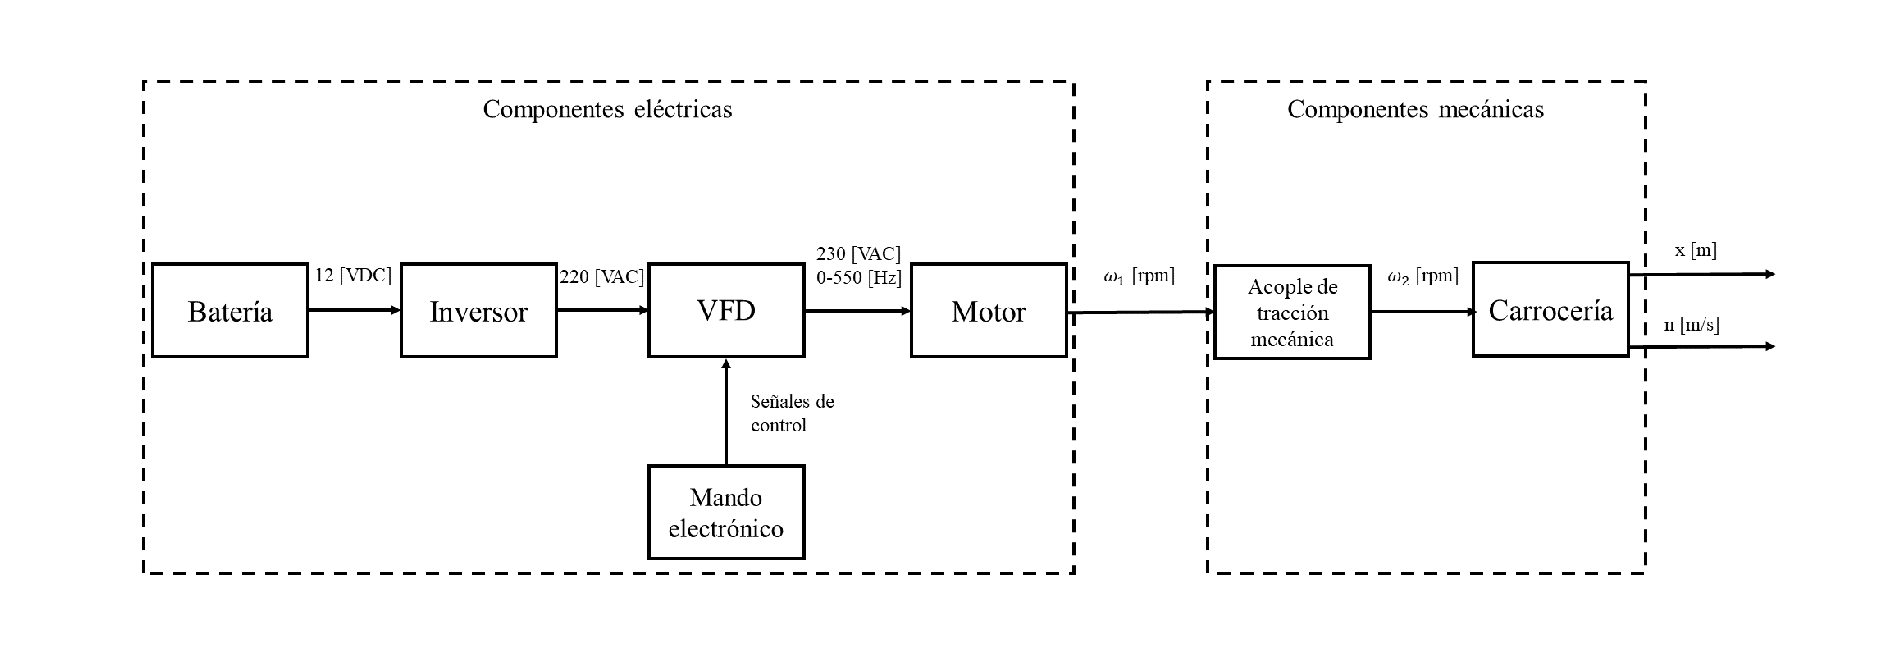
\includegraphics[width=1.05\textwidth]{Figs/PROYECTO_EV.eps}
\caption{Diagrama de bloques funcional para el prototipo de veh�culo}\label{Diagrama_bloques}
\end{figure}
% ------------------------------------------------------------------------
\subsection{Carrocer�a}
% ------------------------------------------------------------------------
Esta parte del sistema corresponde con un armaz�n met�lico que soporta el peso del tren de potencia y el conductor del veh�culo. La Fig. \ref{carroceria} muestra una carrocer�a t�pica, cuyas variaciones a nivel comercial incluyen (entre otras) las de tipo: \emph{sedan}, \emph{hatchback} y \emph{station wagon} \cite{cascajosa2005ingenieria}. Evidentemente, dise�ar una carrocer�a requiere el dominio de conocimientos m�s all� de la base conceptual de un ingeniero electricista o electr�nico, y por tanto, se estableci� contacto con profesores de la Escuela de Ingenier�a Mec�nica (EIM) de la Universidad Industrial de Santander (UIS) para acceder a dise�os de prototipos para competencias (del tipo \emph{VTH}) o adecuar el chasis de veh�culos a gasolina preexistentes. Sin embargo, ninguna de dichas opciones se consider� viable dados los costos de inversi�n y adecuaci�n en comparaci�n con el presupuesto disponible.\\
% ------------------------------------------------------------------------
\begin{figure}[htbp]
\centering		
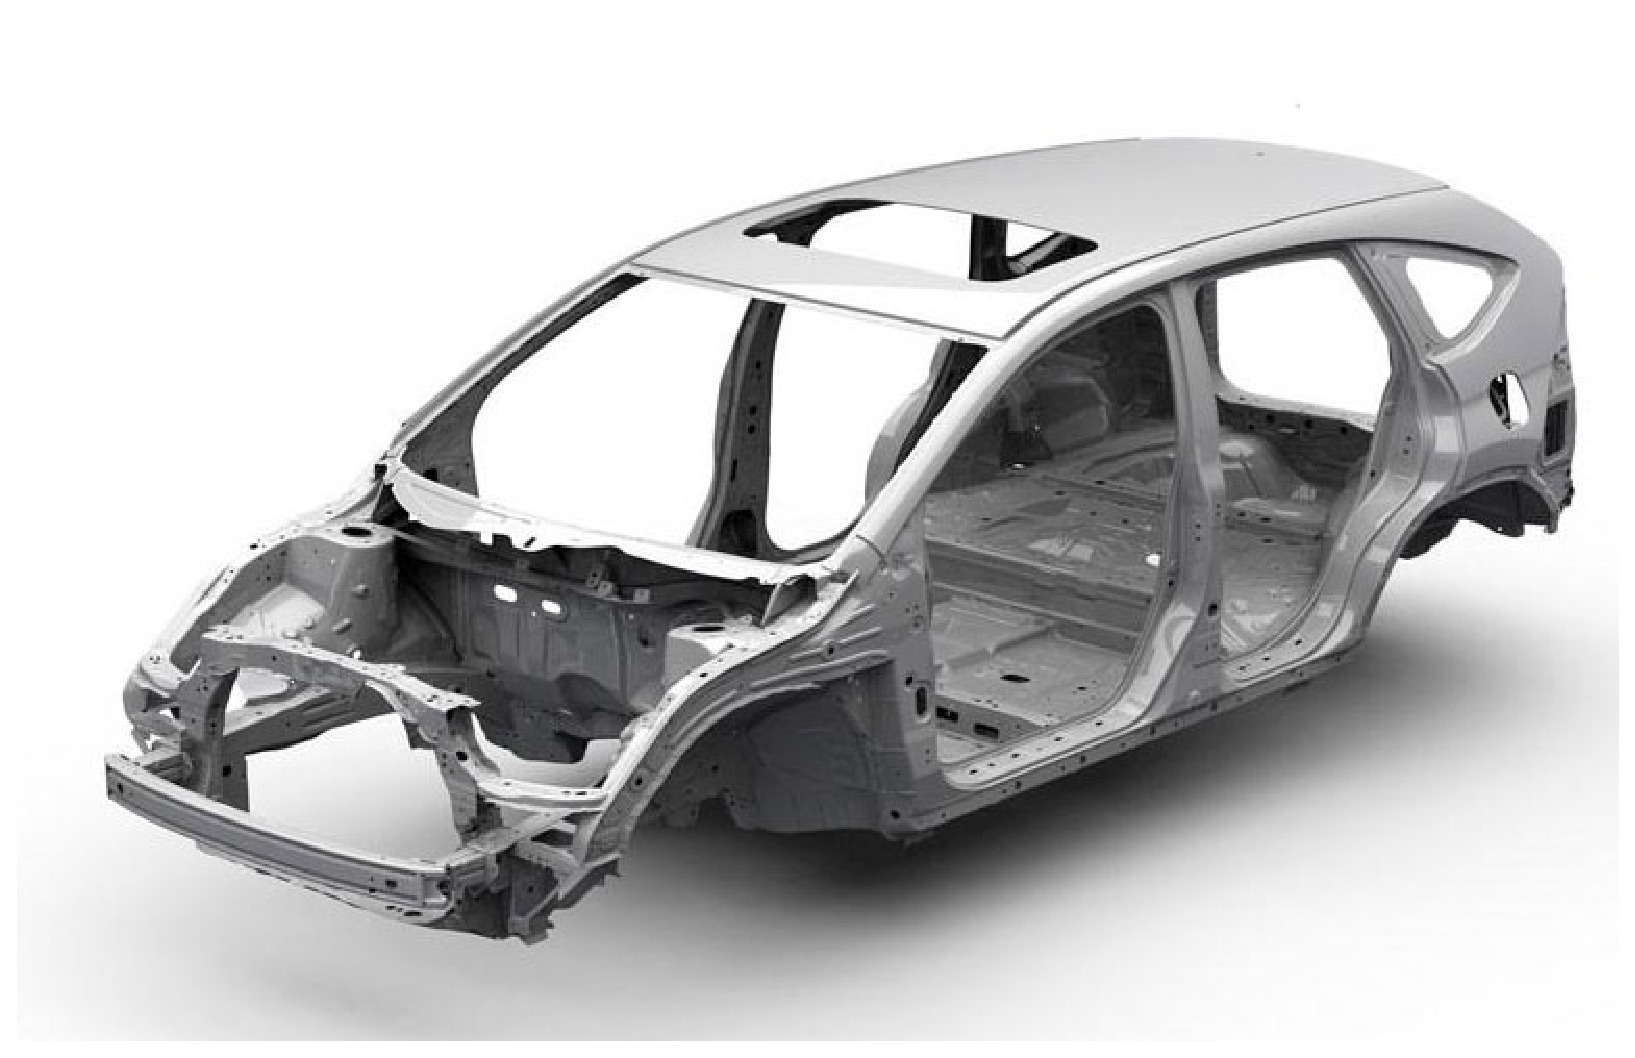
\includegraphics[width=0.5\textwidth]{Figs/carroceria.eps}
\caption{Ilustraci�n para carrocer�a de un veh�culo}\label{carroceria}
\end{figure}
% ------------------------------------------------------------------------

Como alternativa, se adquiri� (por parte de uno de los autores del trabajo de grado) un chasis \emph{VTH} de segunda mano con la apariencia original mostrada en la Fig. \ref{Carroceria_final}. En adelante, se denominar� \emph{chasis} a la parte interna de una carrocer�a.\\
% ------------------------------------------------------------------------
\begin{figure}[htbp]
\centering		
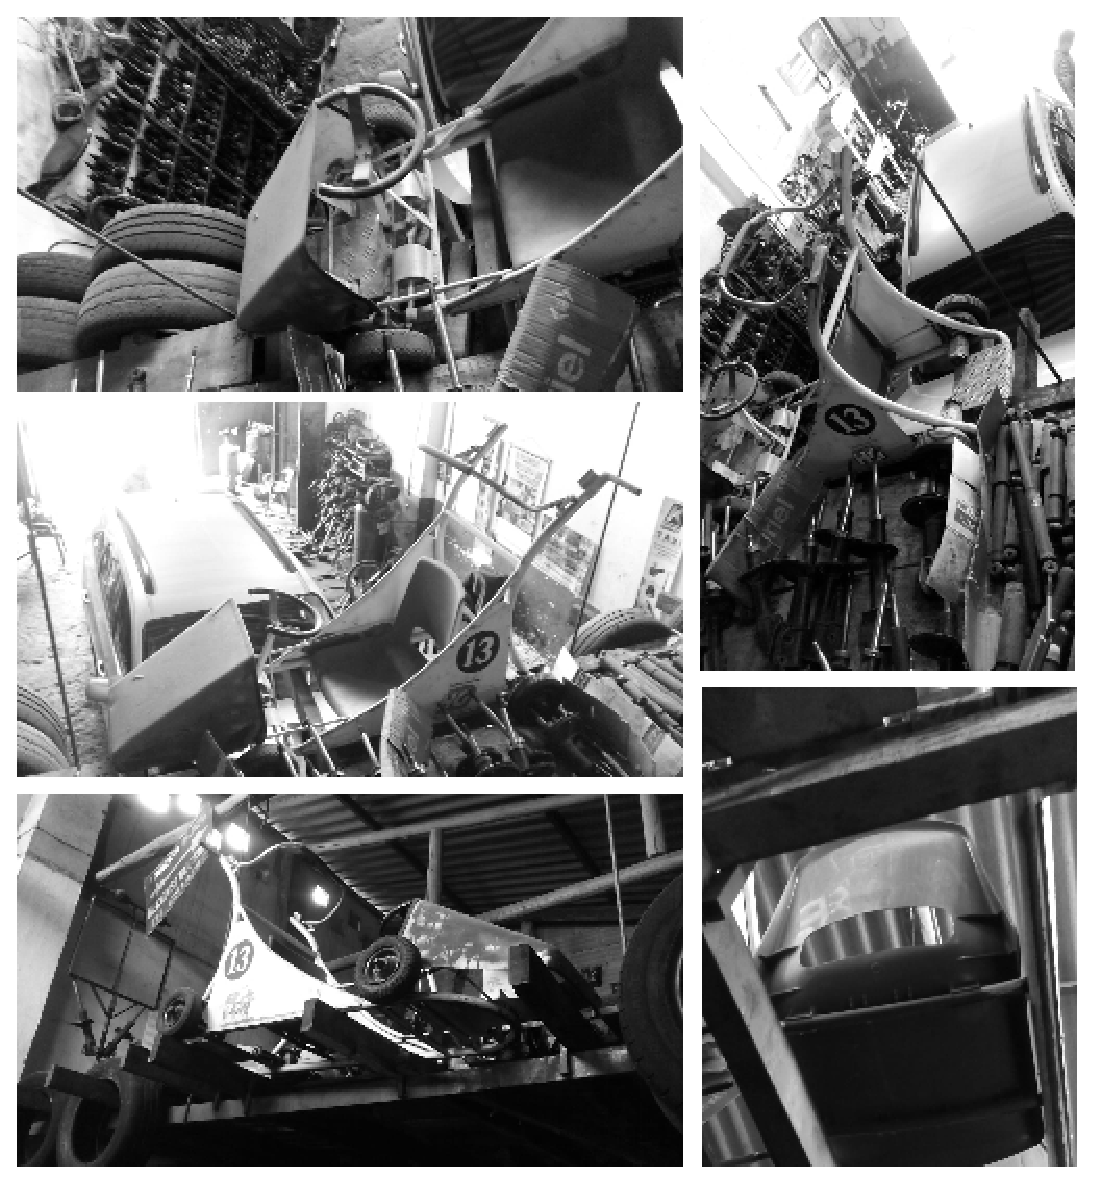
\includegraphics[width=0.9\textwidth]{Figs/Carroceria-final.eps}
\caption{Chasis \emph{VTH} adquirido para el trabajo de grado}\label{Carroceria_final}
\end{figure}
% ------------------------------------------------------------------------

Entre las caracter�sticas principales del chasis adquirido se tienen: un peso de 20 [kg] aproximadamente, una estructura construida en aluminio, frenado por fricci�n mec�nica y un tim�n acondicionado a un mecanismo de direcci�n por palancas. Detalles de la geometr�a del veh�culo y sus dimensiones se presentan en el s�lido tridimensional ilustrado en la Fig. \ref{3D}, construido a partir de la herramienta \texttt{Blender} (\texttt{www.blender.org}).
% ------------------------------------------------------------------------
\begin{figure}[htbp]
\centering
		\subfigure[Vista superior]{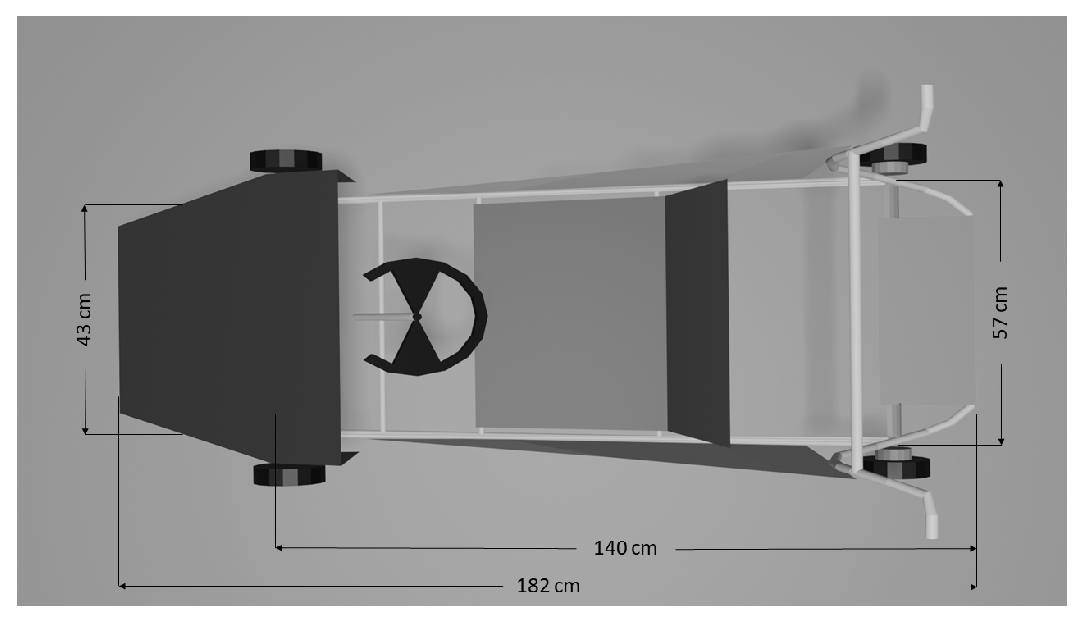
\includegraphics[width=0.6\textwidth]{Figs/Medidas-carro-arriba.eps}}\\
		\subfigure[Vista lateral derecha]{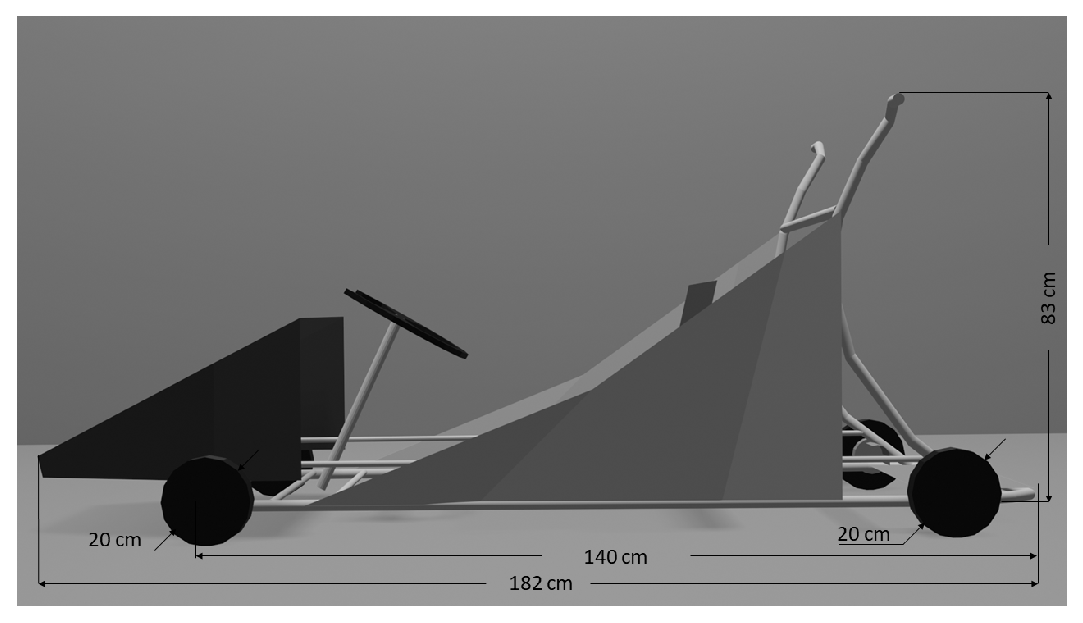
\includegraphics[width=0.6\textwidth]{Figs/Medidas-carro-lado.eps}}
		\caption{Modelo tridimensional con medidas}\label{3D}
\end{figure}
% ------------------------------------------------------------------------
\subsection{Motor el�ctrico}
% ------------------------------------------------------------------------
El coraz�n del \emph{tren de potencia} corresponde con el \emph{motor el�ctrico}. Para dimensionarlo, es necesario calcular la potencia de la carga mec�nica a vencer para producir el movimiento del veh�culo.\\

Lo anterior se realiz� siguiendo las indicaciones de \emph{Ricardo Alfonso Jaimes Rol�n} (Profesor adscrito a la EIM-UIS) y las \emph{Secciones 2.2/2.3} de \cite{ehsani2018modern} ante las siguientes consideraciones:
% ------------------------------------------------------------------------
\begin{itemize}
\item Operaci�n sobre una superficie plana; es decir, lisa, con buen agarre y pendiente cercana a 0�;
\item Velocidad m�xima $v_{cm}$ de 30 [km/h] $\equiv$ 8.33 [m/s], como restricci�n dada por la \texttt{Ley 1239 de 2008} para circulaci�n en zonas escolares y residenciales como la UIS;
\item Tiempo de aceleraci�n $t_a$ de 30 [s] desde el reposo, para reducir corrientes de arranque y requerimientos de potencia en el motor;
\item Masa total del veh�culo $m_c$ de 220 [kg] distribuida en: 20 [kg] del chasis, 80 [kg] del pasajero y 120 [kg] del tren de potencia;
\item Llantas neum�ticas para uso en carretillas (momento de inercia $I_r$ calculado asumiendo forma en anillo), con datos promedio dados por: masa $m_r$ de 3.5 [kg], radio externo $r_e$ de 0.2 [m] e interno $r_i$ de 0.1 [m];
\item �rea transversal $A$ expuesta al viento de valor 1.0032 [m$^2$] (calculada con la forma de un trapecio) para una velocidad $v_v$ de 1.3889 [m/s] $\equiv$ 5 [km/h] promedio del viento en Bucaramanga (seg�n \texttt{www.windfinder.com}). Este valor es bajo comparado con la velocidad del sonido, lo cual simplifica los an�lisis y c�lculos matem�ticos.
\end{itemize}\
% ------------------------------------------------------------------------

A partir de ello, inicialmente se determina la potencia $P_l$ requerida por el motor para vencer la inercia lineal del veh�culo y llevarlo desde el reposo hasta la m�xima velocidad en el tiempo especificado:
% ------------------------------------------------------------------------
\begin{eqnarray*}
P_l & = & F_l \times v_{cm}\\
    & = & 509 \: [W],
\end{eqnarray*}
% ------------------------------------------------------------------------
siendo $F_l$ la fuerza requerida, definida a su vez como:
% ------------------------------------------------------------------------
\begin{eqnarray*}
F_l & = & m_c \times \left(\frac{v_{cm}}{t_a}\right)\\
    & = & 220 \times \left(\frac{8.33}{30}\right)\\
    & = & 220 \times 0.2777\\
    & = & 61.1 \: [N].
\end{eqnarray*}
% ------------------------------------------------------------------------

De otro lado, la potencia $P_r$ requerida por el motor para vencer la inercia rotacional del veh�culo y llevarlo desde el reposo hasta la m�xima velocidad en el tiempo especificado, puede calcularse como:
% ------------------------------------------------------------------------
\begin{eqnarray*}
P_r & = & \tau_r \left(\frac{v_{cm}}{r_e}\right)\\
    & = & 20.24 \: [W],
\end{eqnarray*}
% ------------------------------------------------------------------------
siendo $\tau_r$ el torque requerido, definido a su vez como:
% ------------------------------------------------------------------------
\begin{eqnarray*}
\tau_r & = & 4 \times I_r \times \left(\frac{\frac{v_{cm}}{r_e}}{t_a}\right)\\
       & = & 4 \times \left(\frac{m_r}{2}\times\left(r_i^2 + r_e^2\right)\right)\times\left(\frac{\frac{v_{cm}}{r_e}}{t_a}\right)\\
       & = & 4 \times \left(\frac{3.5}{2}\times\left((0.1)^2+(0.2)^2\right)\right)\times\left(\frac{\frac{8.33}{0.2}}{30}\right)\\
       & = & 0.486 \: [Nm].
\end{eqnarray*}\
% ------------------------------------------------------------------------

Adicionalmente, se deben considerar potencias de p�rdida por rodadura $P_p$ (i.e. fricci�n por contacto con el suelo) y por arrastre del viento $P_a$. Para el primer caso se tiene:
% ------------------------------------------------------------------------
\begin{eqnarray*}
P_p & = & 4 \times F_p \times v_{cm}\\
    & = & 395.27 \: [W],
\end{eqnarray*}
% ------------------------------------------------------------------------
siendo $F_p$ la fuerza de oposici�n ejercida en el punto de contacto, definida a su vez como:
% ------------------------------------------------------------------------
\begin{eqnarray*}
F_p & = & c_p \times m_c \times g \\
    & = & 0.0055 \times 220 \times 9.8\\
    & = & 11.86 \: [N],
\end{eqnarray*}
% ------------------------------------------------------------------------
para un coeficiente de rodadura $c_p$ seleccionado con valor t�pico para llantas BMX empleadas en veh�culos solares \cite{mohd2014design}. A su vez, para el arrastre aerodin�mico es posible escribir:
% ------------------------------------------------------------------------
\begin{eqnarray*}
P_a & = & F_a \times \left(v_v + v_{cm}\right)\\
    & = & 431 \: [W],
\end{eqnarray*}
% ------------------------------------------------------------------------
siendo $F_a$ la fuerza de oposici�n ejercida por el viento, definida a su vez como \cite{ehsani2018modern}:
% ------------------------------------------------------------------------
\begin{eqnarray*}
F_a & = & \frac{\rho}{2} \times c_a \times A \times \left(v_v + v_{cm}\right)^2 \\
    & = & \frac{1.16}{2} \times 0.81 \times 1.0032 \times \left(1.3889 + 8.33\right)^2\\
    & \approx & 44 \: [N],
\end{eqnarray*}
% ------------------------------------------------------------------------
para un $c_a$ representando un coeficiente de arrastre, tomado de:
% ------------------------------------------------------------------------
\begin{center}
\texttt{http://aerodyn.org/Drag/tables.html}
 \end{center}
% ------------------------------------------------------------------------
para el caso de un veh�culo de competencias. Asimismo, $\rho$ es el valor para la densidad del aire en [kg/m$^3$] a presi�n atmosf�rica y 30 [�C].\\

\noindent Finalmente, la potencia requerida por el motor corresponde con:
% ------------------------------------------------------------------------
\begin{eqnarray*}
P_T & = & P_l + P_r + P_p + P_a\\
    & = & 509 + 20.24 + 395.27 + 431\\
    & = & 1355.51 \: [W] \equiv 1.82 \: [HP] \approx 1491.4 \: [W] \equiv 2 \: [HP],
\end{eqnarray*}
% ------------------------------------------------------------------------
aproximando a valores comerciales.\\

Ahora bien, a nivel comercial es posible adquirir motores el�ctricos de 2 [HP] con diferentes caracter�sticas constructivas. Por tanto, para abaratar costos de compra y reducir mantenimientos del dispositivo, se opt� por un motor de inducci�n trif�sico del tipo jaula de ardilla. A su vez, estos pueden construirse para diferentes caracter�sticas de su relaci�n \emph{par-velocidad} seg�n varias categor�as (NEMA \emph{A}, \emph{B}, \emph{C} o \emph{D}) dependiendo de su aplicaci�n.\\

Particularmente, para el caso de un veh�culo el�ctrico se requiere una m�quina que facilite un alto torque en el momento del arranque, siendo el NEMA tipo \emph{C} la opci�n m�s recomendada. Sin embargo, por restricciones presupuestales y de disponibilidad comercial se seleccion� un motor SIEMENS NEMA tipo \emph{B} de referencia 1LE0141-0EB46-4AA4-Z D80+ con las caracter�sticas t�cnicas mostradas en la Tabla \ref{motorparam} y la apariencia f�sica ilustrada en la Fig. \ref{motor}.\\
% ------------------------------------------------------------------------
\begin{table}[htbp]
% ------------------------------------------------------------------------
\centering
\caption{Caracter�sticas t�cnicas de motor}
{\renewcommand{\arraystretch}{0.8}
\begin{tabular}{ll}
% ------------------------------------------------------------------------
\hline
Par�metro               & Valor                                                            \\
\hline
Potencia nominal        & 2 [HP]                                                           \\
Velocidad nominal       & 1720 [rpm]                                                       \\
Torque nominal          & 8.3 [Nm]                                                         \\
Frecuencia de operaci�n & 60 [Hz]                                                          \\
Tensi�n nominal         & 220 $\Delta \Delta$ / 380 $\lambda \lambda$ / 440 $\Delta$ [VAC] \\
Corriente nomunal       & 5.8 $\Delta \Delta$ / 3.35 $\lambda \lambda$ / 2.9 $\Delta$ [A]  \\
Corriente de arranque   & 6 [Ia/In]                                                        \\
Torque de arranque      & 2.6 [Ta/Tn]                                                      \\
Factor de potencia      & 0.81 [\%]                                                        \\
Eficiencia              & Alta (IE2)                                                       \\
\hline
% ------------------------------------------------------------------------
\end{tabular}\label{motorparam}}
% ------------------------------------------------------------------------
\end{table}
% ------------------------------------------------------------------------
\begin{figure}[htbp]
\centering		
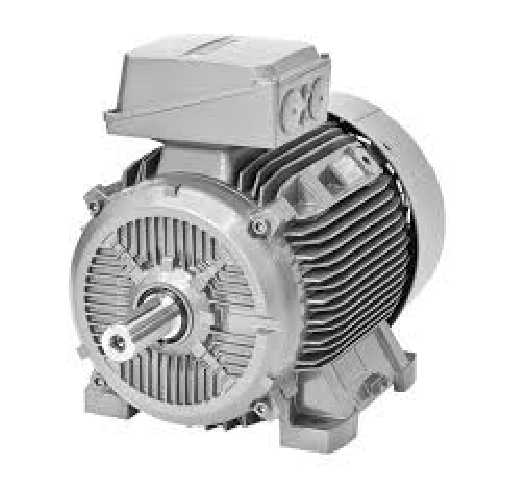
\includegraphics[width=0.4\textwidth]{Figs/motor.eps}
\caption{Motor de inducci�n seleccionado}\label{motor}
\end{figure}
% ------------------------------------------------------------------------

Una vez seleccionado el motor el�ctrico, es posible proceder con la determinaci�n de los elementos
encargados de suministrar para el mismo la potencia el�ctrica de alimentaci�n y la capacidad
de manejo para sus condiciones operativas.
% ------------------------------------------------------------------------
\subsection{Variador de frecuencia}\label{vfdsect}
% ------------------------------------------------------------------------
Un variador de frecuencia o VFD (\emph{Variable-Frequency Drive}) es un dispositivo encargado de modificar las condiciones de alimentaci�n de un motor de inducci�n para alterar su operaci�n. En particular, un VFD mantiene constante el par de la m�quina en un rango de velocidades de inter�s ajustando valores de voltaje y frecuencia de alimentaci�n con relaci�n (V/f) constante. Esto �ltimo se conoce com�nmente como \emph{control escalar}.\\

El primer dato a considerar para elegir el variador es la potencia y el tipo de alimentaci�n del motor; es decir: 2 [HP], 220 [VAC] trif�sico. Estas deben ser las caracter�sticas de salida del VFD.\\

Asimismo, la mayor parte de los VFD comerciales ofrecen la posibilidad de realizar un frenado electr�nico. Entre las modalidades disponibles se pueden mencionar: frenados tipo rampa con par�metros ajustables, por desconexi�n de alimentaci�n (tambi�n denominado \emph{coast}) y din�mico mediante una resistencia externa. Estas opciones de frenado electr�nico se complementan con el frenado mec�nico disponible en el chasis del veh�culo, para garantizar la seguridad del conductor y de las personas en su entorno.\\

Adicionalmente, tomando en cuenta la aplicaci�n particular considerada para el VFD, se requiere que este posea la caracter�stica de mando remoto para activar sus funciones operativas desde la comodidad de un panel localizado en el volante del veh�culo.\\

De esta manera, dentro de las opciones comerciales disponibles en el mercado que satisfacen los requerimientos anteriores se eligi� el variador SIEMENS \emph{Sinamics V20}, con caracter�sticas t�cnicas resumidas en la Tabla \ref{variadorparam}.\\

La conexi�n y configuraci�n de operaci�n (en modo local y remoto) para el dispositivo, ser�n abordadas con detalle en \emph{Secciones} posteriores del presente documento.
% ------------------------------------------------------------------------
\begin{table}[htbp]
% ------------------------------------------------------------------------
\centering
\caption{Caracter�sticas t�cnicas de VFD}
{\renewcommand{\arraystretch}{0.8}
\begin{tabular}{ll}
% ------------------------------------------------------------------------
\hline
Par�metro           & Valor                         \\
\hline
Fases de entrada    & 1                             \\
Tensi�n de red      & 200 ... 240 [V] -15\% +10\%   \\
Frecuencia de red   & 47 ... 63 [Hz]                \\
Fases de salida     & 3                             \\
Tensi�n de carga    & 230 [V]                       \\
Potencia nominal    & 1.50 [kW] / 2 [HP]            \\
Corriente nominal   & 7.8 [A]                       \\
Factor de potencia  & 0.72                          \\
Rendimiento         & 0.98                          \\
\hline
Entradas digitales  & 4                             \\
Salidas digitales   & 2                             \\
Entradas anal�gicas & 2                             \\
Salidas anal�gicas  & 1                             \\
Comunicaciones      & USS / Modbus RTU              \\
Opciones de frenado & por resistencia / por rampa / por desconexi�n\\
Comando local       & a trav�s de panel BOP (\emph{basic operator panel}) integrado\\
Comando remoto      & a trav�s de entradas digitales\\
\hline
% ------------------------------------------------------------------------
\end{tabular}\label{variadorparam}}
% ------------------------------------------------------------------------
\end{table}
% ------------------------------------------------------------------------
\begin{figure}[htbp]
\centering		
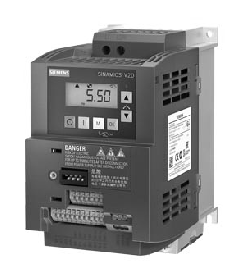
\includegraphics[width=0.3\textwidth]{Figs/Variador.eps}
\caption{VFD seleccionado}\label{variador}
\end{figure}
% ------------------------------------------------------------------------
\subsection{Inversor de potencia}
% ------------------------------------------------------------------------
Un circuito inversor de potencia es un transformador electr�nico que entrega en su salida potencia el�ctrica en corriente alterna ante una entrada
de potencia el�ctrica en corriente continua. Los inversores son circuitos altamente eficientes que pueden alcanzar rendimientos cercanos al 100\% ante ciertas condiciones.\\

A nivel circuital, un inversor est� constituido por arreglos de transistores que operan en modo de conmutaci�n, configurados a partir de diferentes topolog�as como las de \emph{medio puente}, \emph{puente completo} o \emph{flyback}, y que a su vez pueden ser de tipo \emph{monof�sico} o \emph{trif�sico} \cite{rashid2001}. El objetivo del presente trabajo de grado no es abordar en profundidad ese tema espec�fico, ni mucho menos proponer el dise�o de un circuito inversor de potencia y por tanto, la descripci�n se limitar� a justificar la elecci�n de un dispositivo comercial que resuelva las necesidades particulares para este elemento dentro del esquema general para el veh�culo el�ctrico definido previamente en la Fig. \ref{Diagrama_bloques}.\\

M�s a�n, el VFD ya posee como parte importante de su estructura interna un circuito inversor de potencia. Sin embargo, el inversor referido en la presente \emph{Secci�n} corresponde con la interfaz de alimentaci�n entre la fuente principal del sistema y el conjunto \emph{VFD + motor}.\\

Lo anterior impone las siguientes restricciones: 1) la tensi�n de salida del inversor debe ser compatible con la tensi�n de entrada del VFD, 2) la potencia del inversor debe ser al menos la del motor, 3) la entrada del inversor debe ser compatible con los niveles de tensi�n en corriente continua disponibles comercialmente para bater�as en los niveles de potencia de trabajo del sistema.\\

De esta manera, se seleccion� un inversor comercial de marca gen�rica con caracter�sticas t�cnicas mostradas en la Tabla \ref{inversorparam} y apariencia f�sica mostrada en la Fig. \ref{inversor_imagen}.
% ------------------------------------------------------------------------
\begin{table}[htbp]
% ------------------------------------------------------------------------
\centering
\caption{Caracter�sticas t�cnicas del inversor de potencia}
{\renewcommand{\arraystretch}{0.8}
\begin{tabular}{ll}
% ------------------------------------------------------------------------
\hline
Par�metro     	     	& Valor			\\
\hline
Potencia continua  		& 2000 [W]		\\
Potencia pico      		& 4000 [W]		\\
Tensi�n de salida  		& 220 [VAC]		\\
Frecuencia de salida	& 50 [Hz]		\\
Tensi�n de entrada		& 12 [VDC]		\\
Tipo de onda  	 		& Senoidal pura	\\
Puertos de salida  		& 1 monof�sico	\\
\hline
% ------------------------------------------------------------------------
\end{tabular}\label{inversorparam}}
% ------------------------------------------------------------------------
\end{table}
% ------------------------------------------------------------------------
\begin{figure}[htbp]
\centering		
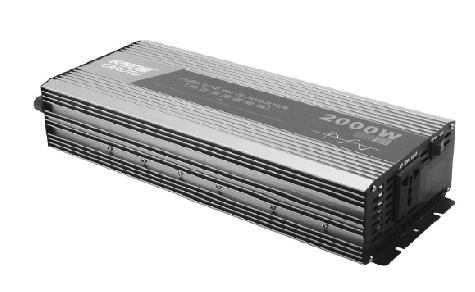
\includegraphics[width=0.5\textwidth]{Figs/Inversor.eps}
\caption{Inversor de potencia seleccionado}\label{inversor_imagen}
\end{figure}
% ------------------------------------------------------------------------
\subsection{Bater�a}
% ------------------------------------------------------------------------
La fuente de energ�a primaria en veh�culos el�ctricos var�a dependiendo de la gama
tecnol�gica y el fabricante. Lo anterior implica que los bancos de bater�as no son
la �nica manera de suministrar la potencia requerida por esta clase de veh�culos, aunque quiz�s
sean todav�a la alternativa m�s popular. Otras opciones incluyen las celdas de combustible y en menor proporci�n
los volantes de inercia, estos �ltimos principalmente para un almacenamiento residual de la energ�a. Ideas m�s osadas pueden incluir veh�culos el�ctricos con celdas solares o miniturbinas y t�neles de viento para capturar energ�a durante su movimiento \cite{ariza2019educational}.\\

Ahora bien, el prototipo a ser implementado utilizar� la opci�n m�s viable desde el punto de vista t�cnico y econ�mico: \emph{bater�as}. No obstante, realizar la elecci�n de una bater�a para un veh�culo el�ctrico implica tener una noci�n (al menos b�sica) de las diferentes gamas y tipos que existen comercialmente para este tipo de producto, evitando as� realizar una mala inversi�n que redunde en el funcionamiento inapropiado de todo el sistema.\\
% ------------------------------------------------------------------------
\begin{figure}[htbp]
\centering		
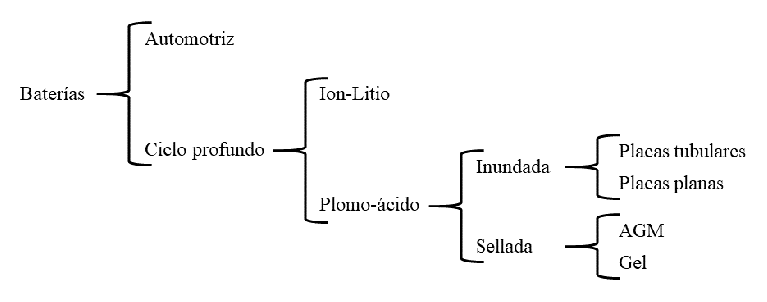
\includegraphics[width=0.8\textwidth]{Figs/Cuadro-sinoptico.eps}
\caption{Cuadro resumen para principales tipos de bater�a}\label{cuadro_sinoptico}
\end{figure}
% ------------------------------------------------------------------------

Al respecto, la Fig. \ref{cuadro_sinoptico} presenta un cuadro sin�ptico que resume a grandes rasgos los tipos principales de bater�as el�ctricas actuales. De ellos, se destaca la de uso \emph{automotriz}, que para este caso no ser�a recomendable debido a que son construidas para proporcionar potencia s�lo en el proceso de ignici�n de veh�culos a gasolina. En constraste, las bater�as de \emph{ciclo profundo} son propicias para trabajo prolongado. Estas a su vez se pueden encontrar en versiones de \emph{Plomo-�cido} y \emph{I�n-Litio}, de las cuales la segunda posee desempe�o superior pero tambi�n es mucho m�s costosa. Por su parte en las \emph{Plomo-�cido} pueden distinguirse dos subcategor�as: la \emph{inundadas} (de placas tubulares o planas) y las \emph{selladas} (en AGM o Gel). La desventaja de las \emph{inundadas} radica en su constante necesidad de mantenimiento, incluso requiriendo agregar agua destilada. Por su parte en el caso de las \emph{selladas} la tecnolog�a \emph{Gel} suele degradarse cuando se expone a altas temperaturas.\\

Por tanto, los argumentos anteriores permiten concluir que una bater�a de \emph{ciclo profundo}, \emph{Plomo-�cido}, \emph{sellada} y del tipo \emph{AGM} (separador de vidrio absorbente) representa la opci�n tecnol�gica m�s adecuada a ser implementada como fuente primaria principal del prototipo de veh�culo el�ctrico.\\

De esta manera siendo la potencia del motor 2 [HP] $\approx$ 1500 [W] y tomando en cuenta las restricciones en la tensi�n de corriente continua a la entrada del inversor de potencia, la corriente proporcionada por la bater�a (ante un escenario de elementos ideales y m�xima carga) deber� ser:
% ------------------------------------------------------------------------
$$
\frac{1500 \: [W]}{12 \: [VDC]} = 125 \: [A].
$$\
% ------------------------------------------------------------------------

Comercialmente, fue posible adquirir una bater�a NETION de ciclo profundo AGM de 12 [VDC] / 150 [Ah] con caracter�sticas adicionales mostradas en la Tabla \ref{bateriaparam} y apariencia f�sica seg�n la Fig. \ref{bateria_imagen}. A partir de ello, se aspira satisfacer la operaci�n del sistema en un rango de m�xima carga por un tiempo prolongado (de al menos 30 minutos). Adicionalmente, se adquiri� un cargador de bater�as gen�rico con apariencia similar a la mostrada en la Fig. \ref{cargador} que supone un tiempo total de carga de 6 horas.
% ------------------------------------------------------------------------
\begin{table}[htbp]
% ------------------------------------------------------------------------
\centering
\caption{Caracter�sticas t�cnicas de bater�a}
{\renewcommand{\arraystretch}{0.8}
\begin{tabular}{ll}
% ------------------------------------------------------------------------
\hline
Par�metro     	     					& Valor					\\
\hline
Resistencia interna a carga completa	& 3.5 [m$\Omega$]		\\
M�xima pendiente de descarga     		& 1200 [A] / 5 [s]		\\
Corriente de carga m�xima				& 45 [A]				\\
Autodescarga (25 �C, 12 meses)  		& 35\% 					\\
Dimensiones (Largo x Ancho x Alto)		& 485 x 172 x 240 [mm]	\\
Peso aproximado 						& 45.5 [kg]				\\
\hline
% ------------------------------------------------------------------------
\end{tabular}\label{bateriaparam}}
% ------------------------------------------------------------------------
\end{table}
% ------------------------------------------------------------------------
\begin{figure}[htbp]
\centering
		\subfigure[Bater�a]{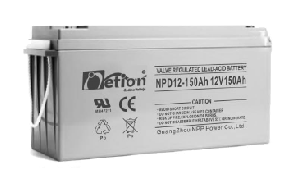
\includegraphics[width=0.4\textwidth]{Figs/Bateria.eps}\label{bateria_imagen}}\\
		\subfigure[Cargador]{\includegraphics[width=0.4\textwidth]{Figs/Cargador.eps}\label{cargador}}
		\caption{Bater�a y cargador de bater�a seleccionados}
\end{figure}
% ------------------------------------------------------------------------
\subsection{Acople de tracci�n mec�nica}
% ------------------------------------------------------------------------
Para transferir la potencia mec�nica del motor el�ctrico a la carga mec�nica
representada por las partes del veh�culo el�ctrico, se realiz� un acople mec�nico.\\

Inicialmente, respetando el dise�o original del chasis del veh�culo
se conserv� la tracci�n en las ruedas traseras. A partir de ello, se analizaron diferentes opciones para ejecutar la interconexi�n entre el eje del motor el�ctrico y el eje de las ruedas, siendo quiz�s la m�s apropiada una caja reductora de engranajes c�nicos que permitiese, adem�s de un acople sin p�rdidas, ubicar el motor en posici�n ortogonal al eje de rotaci�n de las ruedas para mejorar el aprovechamiento de espacio. Sin embargo, al momento de cotizar este tipo de acople se encontr� que superaba notablemente las expectativas de presupuesto del proyecto y por tanto, se propuso una soluci�n alternativa y m�s econ�mica, correspondiente con dos ruedas dentadas (engranajes) y un acople a trav�s de cadena como el ilustrado en la Fig. \ref{cadena}.\\
% ------------------------------------------------------------------------
\begin{figure}[htbp]
\centering		
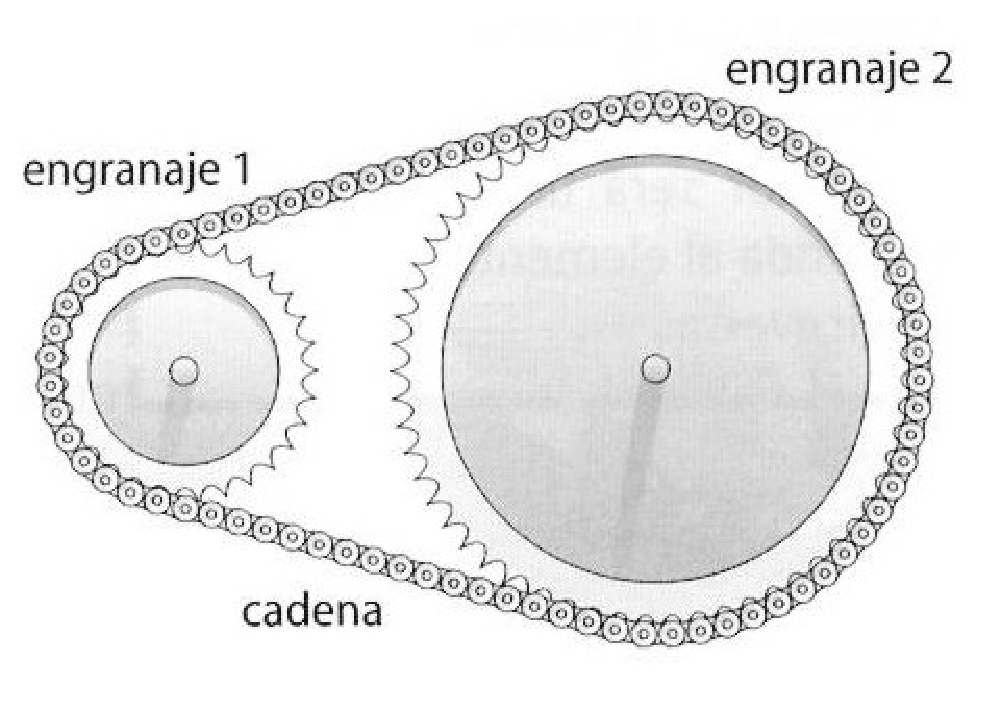
\includegraphics[width=0.4\textwidth]{Figs/cadena.eps}
\caption{Acople de engranajes por cadena}\label{cadena}
\end{figure}
% ------------------------------------------------------------------------

Para realizar el dimensionamiento de los engranajes, se consider� la relaci�n de transformaci�n $N$ a m�xima velocidad:
% ------------------------------------------------------------------------
\begin{eqnarray*}
N &=& \frac{\omega_2}{\omega_1} = \frac{v_{cm} \: [rpm]}{1720 \: [rpm]}\\
  &=& \frac{ \left( \frac{8.33 \: [m/s]}{2 \times \pi \times r_e \: [m/rev]} \times \frac{60 \: [s]}{1 \: [min]}\right)}{1720 \: [rpm]}\\
  &=& \frac{ \left( 6.6288 \: [rev/s] \times \frac{60 \: [s]}{1 \: [min]}\right)}{1720 \: [rpm]}\\
  &=& \frac{397.73 \: [rpm]}{1720 \: [rpm]} = 0.23 \approx \frac{1}{5},
\end{eqnarray*}
% ------------------------------------------------------------------------
ante una operaci�n de motor a velocidad nominal.\\

A partir de ello, se acudi� a un taller de metalmec�nica para construir dos ruedas de acero inoxidable, una con 9 dientes (equivalentes a 2 [cm] de radio) acoplada el eje del motor y otra con 45 dientes (equivalentes a 10 [cm] de radio) acoplada al eje de las ruedas. Asimismo, se emple� una cadena de acero de 95 [cm] de largo para una distancia efectiva entre ejes de 30 [cm] aproximadamente. El montaje final para el acople de tracci�n mec�nica se visualiza en la Fig. \ref{cadena_pinones}.
% ------------------------------------------------------------------------
\begin{figure}[htbp]
\centering		
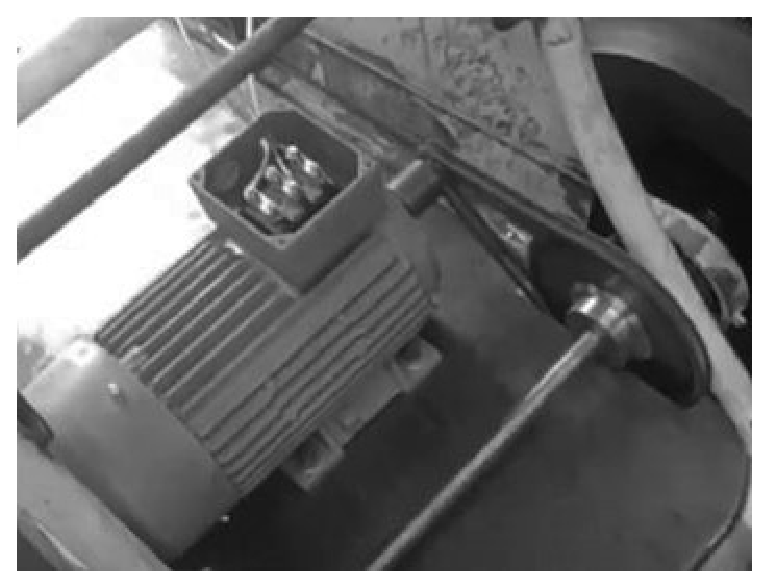
\includegraphics[width=0.45\textwidth]{Figs/cadena_pinones.eps}
\caption{Acople real implementado en el veh�culo}\label{cadena_pinones}
\end{figure}
% ------------------------------------------------------------------------
\section{Adecuaciones mec�nicas}
% ------------------------------------------------------------------------
El chasis adquirido para el desarrollo del proyecto (previamente mostrado en las Figs. \ref{Carroceria_final} y \ref{3D}) fue construido con un prop�sito diferente al de un veh�culo el�ctrico, y por tanto, fue necesario acondicionar dicha estructura de base para tener un mejor desempe�o desde el punto de vista m�canico (motr�z) y ergon�mico. As�, adicional al acople de tracci�n mec�nica explicado en la \emph{Secci�n} anterior, se definieron y ejecutaron las siguientes adecuaciones:
% ------------------------------------------------------------------------
\begin{itemize}
\item[a)] \emph{Utilizar un nuevo conjunto de ruedas que soporte el peso del chasis, el pasajero y de todos los dispositivos el�ctricos a ser agregados}. Para ello se incluyeron 4 ruedas neum�ticas de 40 [cm] de di�metro y con capacidad de soportar hasta 150 [kg] cada una. La Fig. \ref{rueda} ilustra la apariencia f�sica de las ruedas utilizadas;
% ------------------------------------------------------------------------
\begin{figure}[htbp]
\centering		
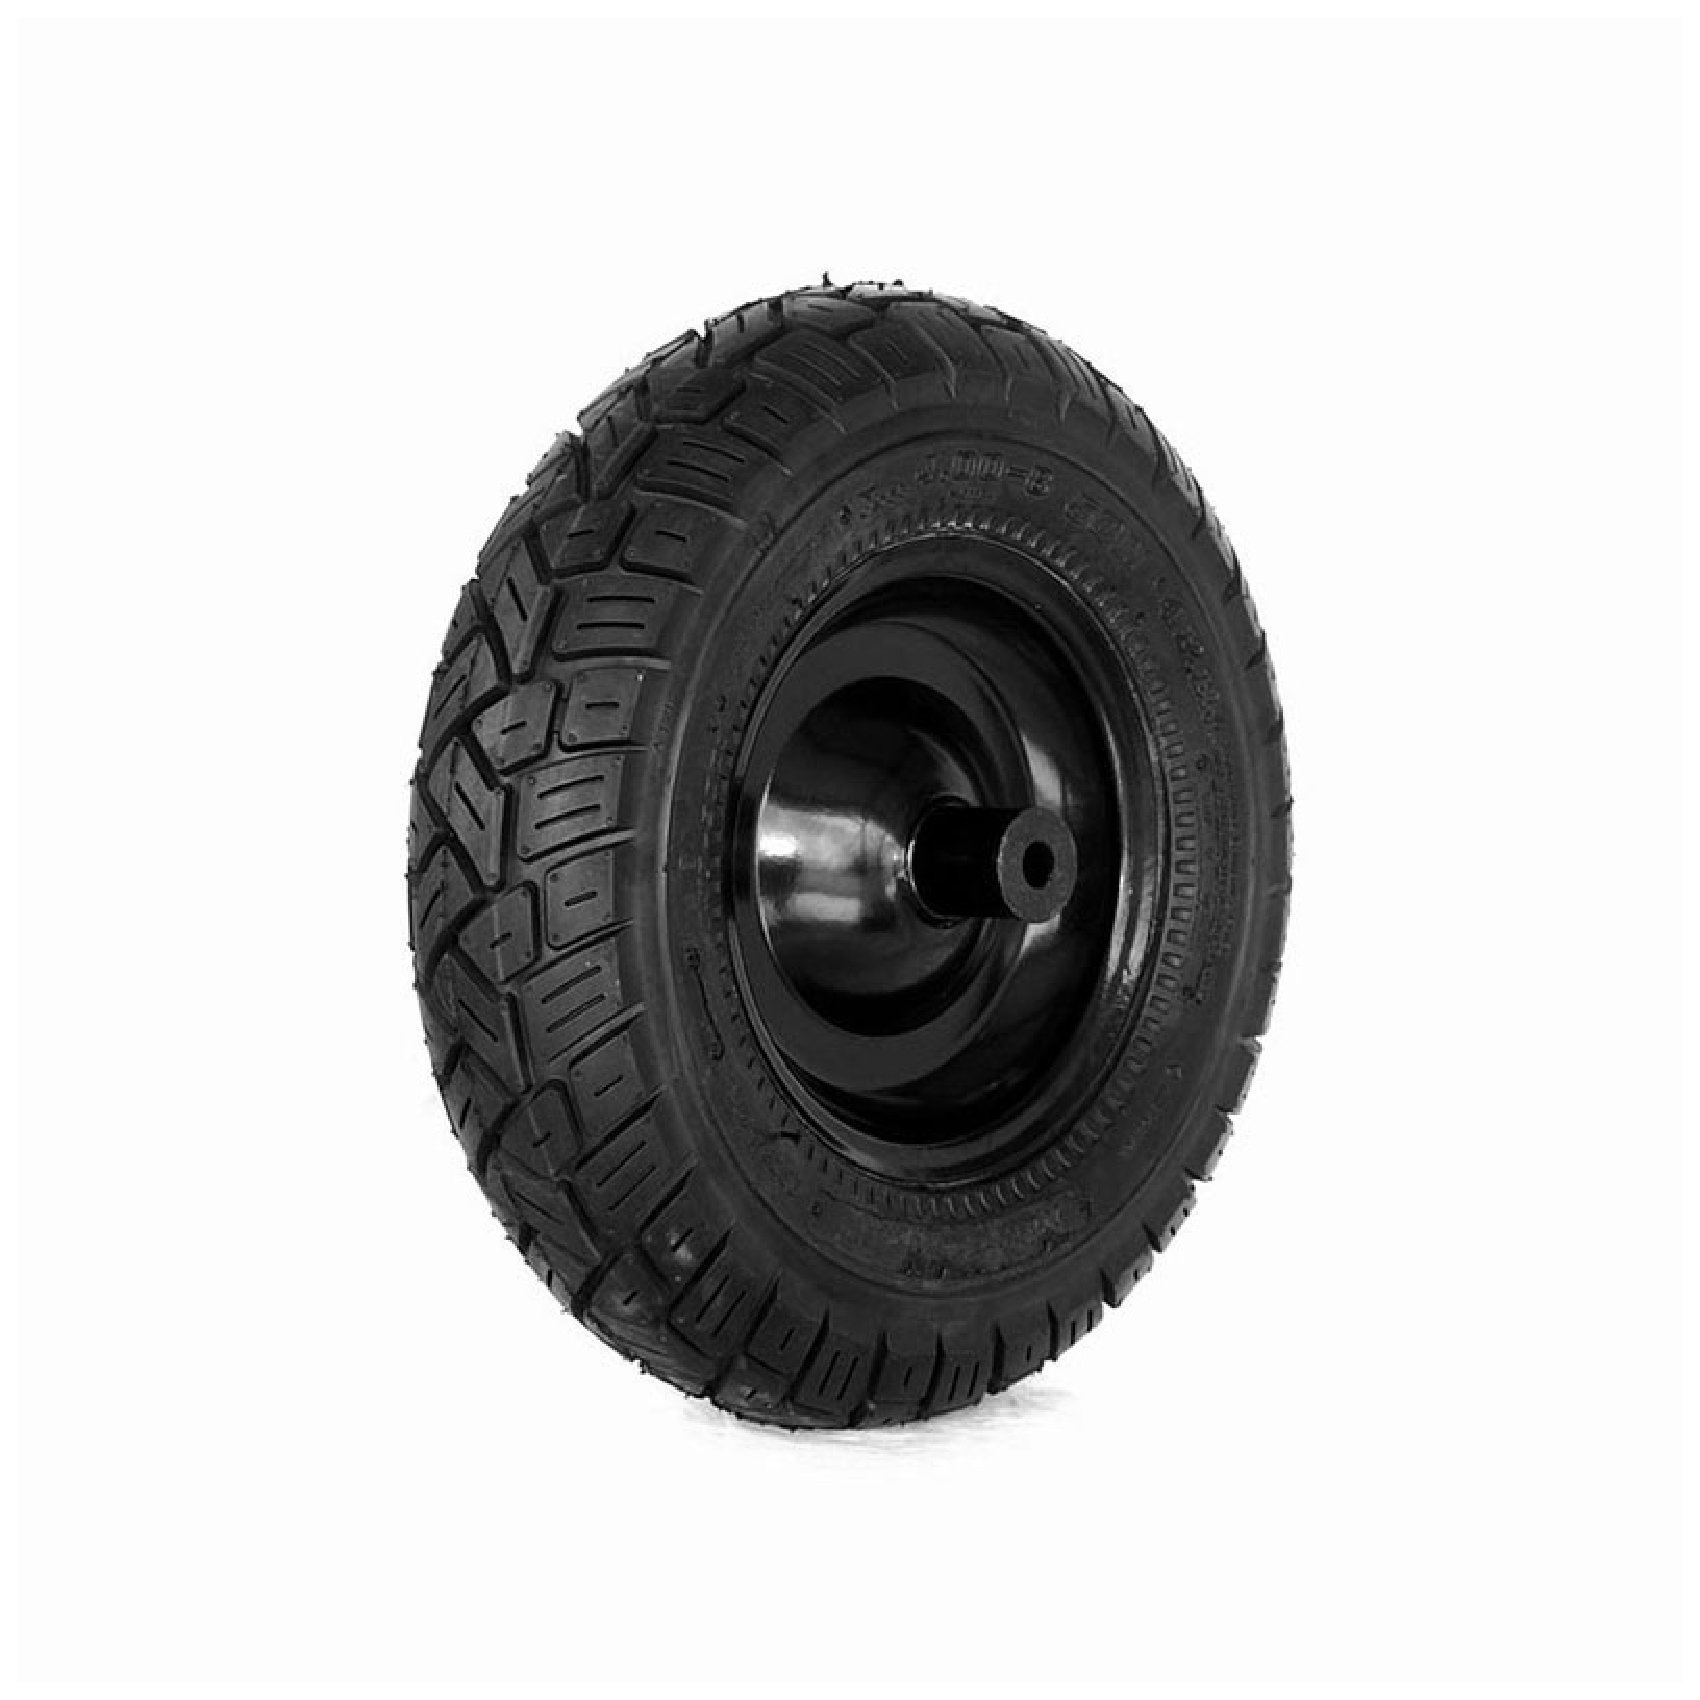
\includegraphics[width=0.3\textwidth]{Figs/rueda.eps}
\caption{Rueda neum�tica seleccionada}\label{rueda}
\end{figure}
% ------------------------------------------------------------------------
\item[b)] \emph{Realizar el acople de las ruedas con los ejes delantero y trasero del veh�culo}. En particular, las ruedas empleadas poseen un acople tipo macho y debido a esto fue necesario acondicionar un rodamiento mediante chumaceras (balineras troqueladas de 5/8'') para facilitar el movimiento de cada eje. Para el caso de las ruedas delanteras, un extremo de la chumacera fue soldado al acople mientras el otro fue asegurado por tornillos al mecanismo de giro (direcci�n), permitiendo un movimiento libre e independiente de cada eje delantero (izquierdo y derecho). Por su parte, las ruedas traseras fueron conectadas a trav�s de un tornillo al v�stago del eje en el punto de acople. Posteriormente, dicho v�stago fue acoplado a la cara interna de dos chumaceras equidistantes a lo largo de su longitud, con el extremo externo de las chumaceras asegurado por tornillos al chasis del veh�culo. De esta manera se obtuvo un rodamiento sin fricci�n ni vibraciones al momento de aplicarse tracci�n mec�nica por parte de los engranajes. La Fig. \ref{rodamientos} ilustra la apariencia f�sica de los rodamientos utilizados;
% ------------------------------------------------------------------------
\begin{figure}[htbp]
\centering		
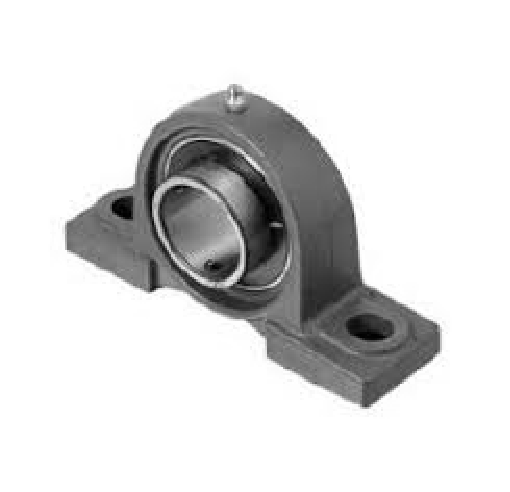
\includegraphics[width=0.25\textwidth]{Figs/balinera.eps}
\caption{Rodamientos empleados en adecuaciones}\label{rodamientos}
\end{figure}
% ------------------------------------------------------------------------
\item[c)] \emph{Utilizar una placa r�gida en la base del veh�culo para soportar el peso de los elementos el�ctricos seleccionados en el tren de potencia}. Para este prop�sito se emple� una l�mina de aluminio (lisa) de 2.5 [mm] de espesor y 5200 [cm$^2$] de �rea aproximadamente (un trapecio con bases de 54.5 [cm] y 40.5 [cm], y altura 110 [cm]);
\item[d)] \emph{Modificar las proporciones de espacio del pasajero al interior de la cabina}. En este caso se realizaron tres modificaciones principales: i) incrementar la altura del asiento (34 [cm] desde su posici�n original), ii) mover el asiento hacia atr�s hasta el m�ximo tope permitido por la estructura (travesa�o trasero) y iii) ajustar la altura del volante a la nueva altura del asiento de manera tal que existieran 20 [cm] de espacio entre ellos para facilitar la movilidad de las piernas del conductor;
\item[e)] \emph{Incrementar el �ngulo de maniobra de giro para las ruedas delanteras}. Los ajustes descritos previamente para el acople de las ruedas delanteras al mecanismo de giro (direcci�n), permitieron obtener una distancia de alrededor 10 [cm] entre el chasis del veh�culo y los ejes de las ruedas, facilitando realizar maniobras de giro con �ngulo suficiente (de hasta 30�) durante la conducci�n. Este aspecto es relevante, pues al momento de seleccionar un nuevo conjunto de ruedas no hab�a garant�a que las mismas se ajustaran apropiadamente al dise�o original del veh�culo;
\item[f)] \emph{Realizar limpieza y pintura del chasis modificado}. Para ello se emple� pintura electrost�tica de color \texttt{verde 6018}, que identifica a la Universidad Industrial de Santander;
\item[g)] \emph{Distribuir los elementos el�ctricos del tren de potencia en la geometr�a del veh�culo modificado}. Sobre la base del modelo tridimensional presentado en la Fig. \ref{Modelo_Blender_2}, se realiz� la distribuci�n espacial para los elementos principales del tren de potencia que representan las componentes el�ctricas del diagrama de bloques definido en la Fig. \ref{Diagrama_bloques} para el prototipo de veh�culo. La distribuci�n del espacio se realiz� siguiendo el sentido com�n y tratando de combinar aspectos de confort y seguridad para el pasajero;
% ------------------------------------------------------------------------
\begin{figure}[htbp]
\centering		
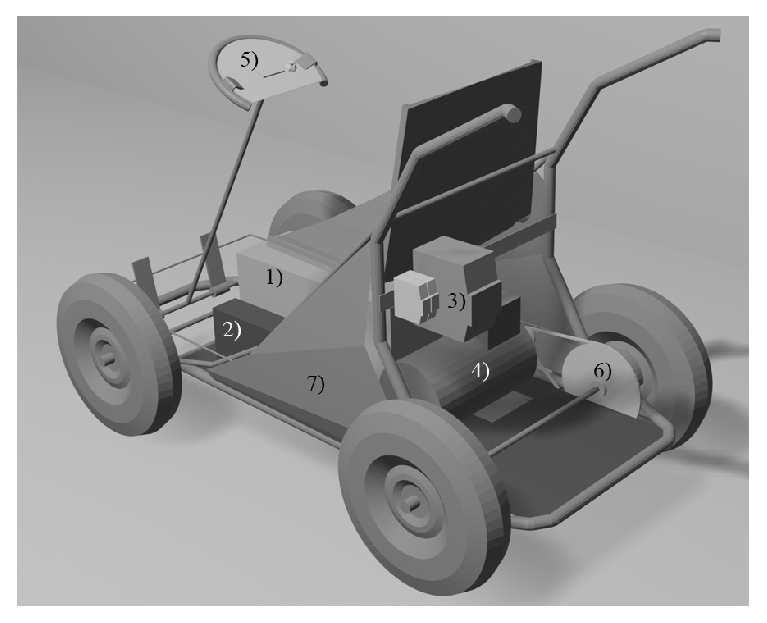
\includegraphics[width=0.5\textwidth]{Figs/Modelo-Blender-Enumerado.eps}
\caption{Modelo tridimensional para ubicaci�n de equipos en veh�culo modificado: 1) bater�a, 2) inversor, 3) VFD, 4) motor, 5) mando electr�nico, 6) acople de tracci�n mec�nica y 7) carrocer�a}
\label{Modelo_Blender_2}
\end{figure}
% ------------------------------------------------------------------------
\item[h)] \emph{Fijaci�n de elementos el�ctricos del tren de potencia al chasis del veh�culo modificado}. Para asegurar la bater�a a la estructura se utilizaron perfiles de aluminio en forma de L (o chapetas) de 1/4'' de grosor, ajustados al per�metro de la forma rectangular y asegurados a la l�mina de base mediante remaches. Usa soluci�n similar fue empleada para el inversor de potencia. Por su parte el motor fue fijado a la l�mina de base empleando tornillos con tuerca de 1/2'' a trav�s de perforaciones alargadas para ajustar la tensi�n mec�nica de la cadena. Finalmente, el variador de velocidad fue atornillado a una placa de aluminio fijada con remaches a un riel omega, a su vez fijado con remaches al travesa�o trasero del veh�culo;
% ------------------------------------------------------------------------
\item[i)] \emph{Dise�o de identidad visual}. Se agregaron logotipos de identidad visual al prototipo de veh�culo el�ctrico, empleando dise�os preexistentes que identifican a la Universidad Industrial de Santander y a la Escuela de Ingenier�as El�ctrica, Electr�nica y de Telecomunicaciones. Adicionalmente, se construy� un logotipo especial para el proyecto denominado por los autores: \texttt{E3carT}. Dichos logotipos se ilustran en la Fig. \ref{Stickers} y fueron adheridos al veh�culo a manera de calcoman�as.
% ------------------------------------------------------------------------
\begin{figure}[htbp]
\centering		

\includegraphics[width=0.3\textwidth]{Figs/sticker.eps}
\caption{Identidad visual para prototipo de veh�culo el�ctrico}\label{Stickers}
\end{figure}
% ------------------------------------------------------------------------
\end{itemize}
% ------------------------------------------------------------------------
\section{Adecuaciones el�ctricas}
% ------------------------------------------------------------------------
La Fig. \ref{cade_simu} muestra la interconexi�n realizada entre los elementos que constituyen las \emph{componentes el�ctricas} del tren de potencia. Dicho diagrama (construido a manera de esquemas de mando y potencia) muestra adem�s de las conexiones, a todos los elementos de accionamiento y protecci�n utilizados.\\
% ------------------------------------------------------------------------
\begin{figure}[htbp]
\centering		
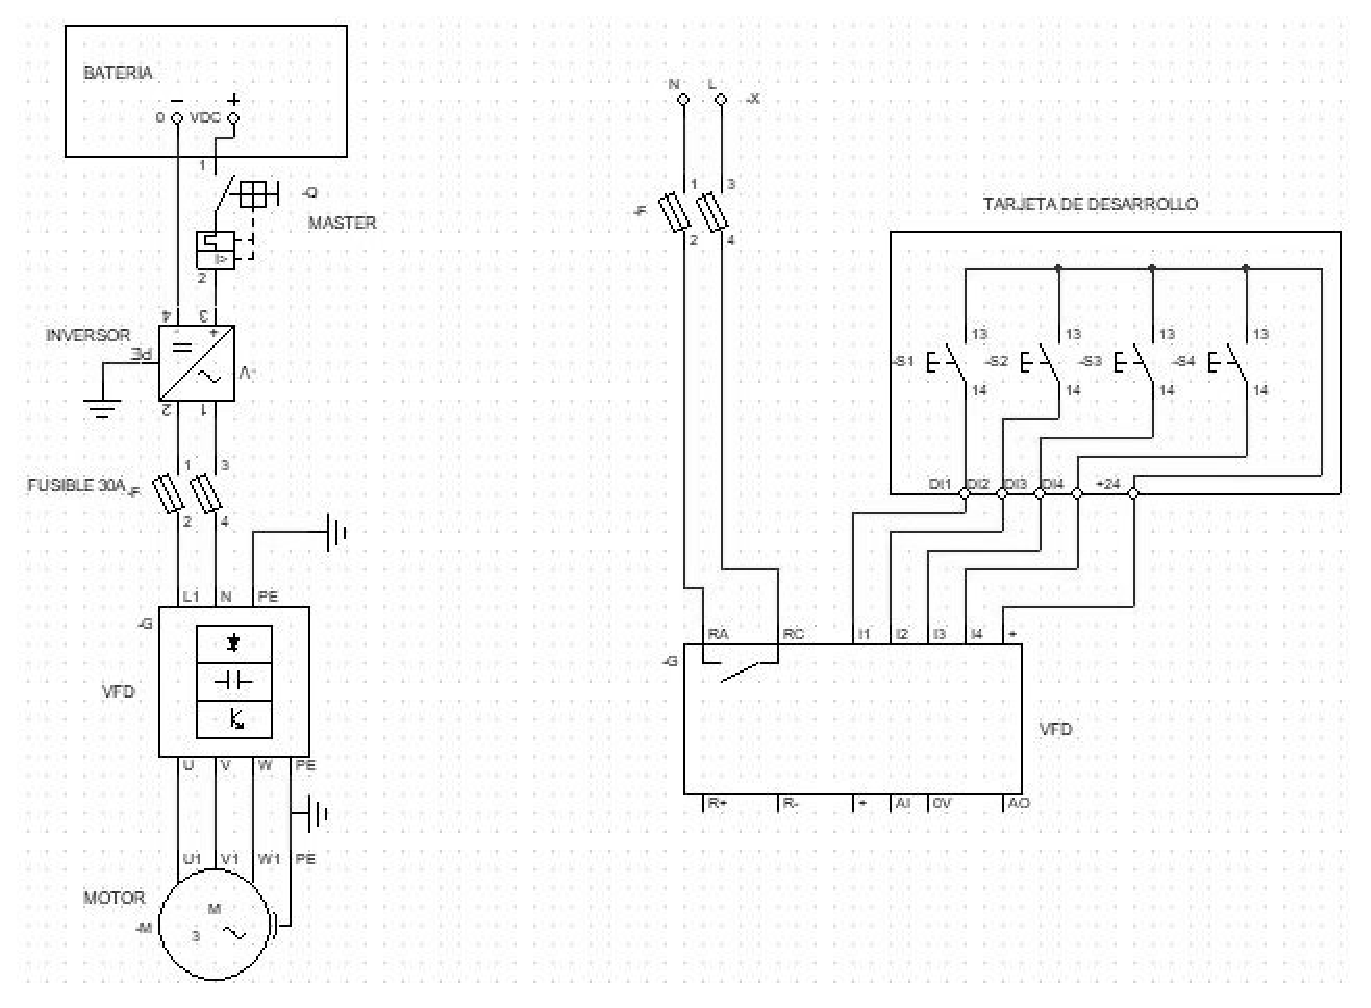
\includegraphics[width=1.0\textwidth]{Figs/circuito_control.eps}
\caption{Esquema de conexiones el�ctricas del prototipo: diagrama de mando (derecha) y potencia (izquierda)}\label{cade_simu}
\end{figure}
% ------------------------------------------------------------------------

De ellos, se destaca el interruptor denominado \texttt{MASTER} que tiene como funci�n desenergizar la alimentaci�n de todos los dispositivos a partir de la desconexi�n de la bater�a. Asimismo, se resalta la inclusi�n de fusibles de 600 [V] / 30 [A] en las l�neas de conexi�n entre el inversor de potencia y el VFD, para proteger los dispositivos ante una sobrecarga. Adicionalmente, se observa la inclusi�n de una \texttt{TARJETA DE DESARROLLO} para realizar el control de operaci�n del sistema seg�n se explicar� con detalle en la siguiente \emph{Secci�n}.\\

Por �ltimo, es conveniente aclarar que la conexi�n a tierra de las componentes el�ctricas del prototipo se realiz� mediante la fijaci�n al chasis de las terminales de tierra monof�sica en la salida del inversor y trif�sica en la salida del VFD.
% ------------------------------------------------------------------------
\section{Adecuaciones electr�nicas}
% ------------------------------------------------------------------------
Hasta el momento, se ha abordado con detalle el dimensionamiento las componentes el�ctricas
y su acople con las componentes mec�nicas del prototipo de veh�culo el�ctrico. Sin embargo, 
a�n no se ha discutido la manera de operar el tren de potencia.\\

Por tanto, a partir del diagrama de bloques de la Fig. \ref{Diagrama_bloques} y de la descripci�n t�cnica para el VFD realizada en la \emph{Subsecci�n} \ref{vfdsect}, es claro que dicho dispositivo constituye la unidad de mando para operaci�n del motor el�ctrico y por ende del tren de potencia del veh�culo.\\

En particular, es posible operar el VFD en modo local a trav�s de la interfaz de usuario (panel BOP - \emph{basic operator panel}) o en modo remoto haciendo uso de sus puertos de entrada anal�gicos y digitales. En cualquier caso, la operaci�n del VFD (y por consiguiente del motor el�ctrico) se realiza posterior a la configuraci�n de par�metros referidos principalmente a los datos de placa del motor.\\ 

A partir de ello, inicialmente se configur� el VFD asignando valores consistentes a dichos par�metros; es decir: tensi�n nominal $P0304 = 220$ [V], corriente nominal $P0305 = 5.8$ [A], potencia nominal $P0307 = 1.5$ [kW], factor de potencia $P0308 = 0.81$, frecuencia nominal $P0310 = 60$ [Hz] y velocidad nominal $P0311 = 1720$ [rpm]. Adicionalmente, se configur� una frecuencia de alimentaci�n para el VFD de 50 [Hz] ($P0100 = 0$).\\

Posteriormente, se procedi� a dise�ar y construir una tarjeta electr�nica para realizar la operaci�n remota del VFD (correspondiente con la \texttt{TARJETA DE DESARROLLO} indicada en el \emph{esquema de mando} de la Fig. \ref{cade_simu}), atendiendo a los siguientes requerimientos:
% ------------------------------------------------------------------------
\begin{itemize}
\item[\emph{1)}] Como elementos de entrada se requieren botones para realizar las maniobras de avance y retroceso, respectivamente;
\item[\emph{2)}] Se requiere un bot�n adicional para ejecutar la maniobra de frenado el�ctrico;
\item[\emph{3)}] Se requiere un medio para detectar por parte del sistema electr�nico la activaci�n del freno mec�nico, ejecutando la maniobra de desconexi�n del tren de potencia el�ctrico. Para ello, se ubic� un sensor del tipo FSR (force sensitive resistor) acoplado mec�nicamente al pedal del freno. De esta manera, la presi�n mec�nica ejercida por el pedal sobre el dispositivo crea una diferencia de potencial el�ctrico en sus terminales constituyendo una se�al anal�gica con niveles de voltaje detectables;
\item[\emph{4)}] Se requiere un indicador para conocer la condici�n de operaci�n del veh�culo a partir de la elecci�n realizada por el usuario en el mando electr�nico. Para este prop�sito se emple� una pantalle de cristal l�quido (LCD) de 16 caracteres y 2 l�neas;
\item[\emph{5)}] Se desea que el sistema electr�nico sea de configuraci�n flexible para adecuarse a futuros requerimientos y funcionalidades adicionales. Tomando en cuenta lo anterior, se utiliz� como unidad de gesti�n de informaci�n al microcontrolador PIC \texttt{18F4550};
\item[\emph{6)}] Para confort del usuario, la unidad electr�nica de mando deber� ubicarse en un lugar estrat�gico dentro del veh�culo. De esta manera, se decidi� localizarla al interior del voltante.
\end{itemize}
% ------------------------------------------------------------------------

El diagrama esquem�tico para el circuito electr�nico dise�ado, incluyendo los elementos mencionados, se presenta en la Fig. \ref{esquema}. A partir de ello, se destaca el acople entre las salidas digitales del microcontrolador y las entradas digitales del VFD a trav�s de optoacopladores (para elevar los niveles de se�al de $5$ [VDC] a $24$ [VDC] \textcolor[rgb]{0.98,0.00,0.00}{\textbf{�De d�nde obtuvieron los $24$ [VDC] si la bater�a es de $12$ [VDC]?RTA:  La alimentacion DC de la PCB esta dada por el VFD el cual tiene una salida de 24, entrada que esta conectada a la PCB por medio del conector $IN24$ mostrado en \ref{esquema}}}, la conversi�n paralelo a serie entre la pantalla LCD y el microcontrolador a trav�s de un convertidor \texttt{I2C} de referencia \texttt{PCF8574} (reduciendo el tama�o del enrutado en la tarjeta) y la regulaci�n de alimentaci�n de 24 [VDC] a 5 [VDC] (para alimentar los elementos del circuito, en su mayor�a de tecnolog�a \texttt{TTL}).\\
% ------------------------------------------------------------------------
\begin{figure}[htbp]
\centering		
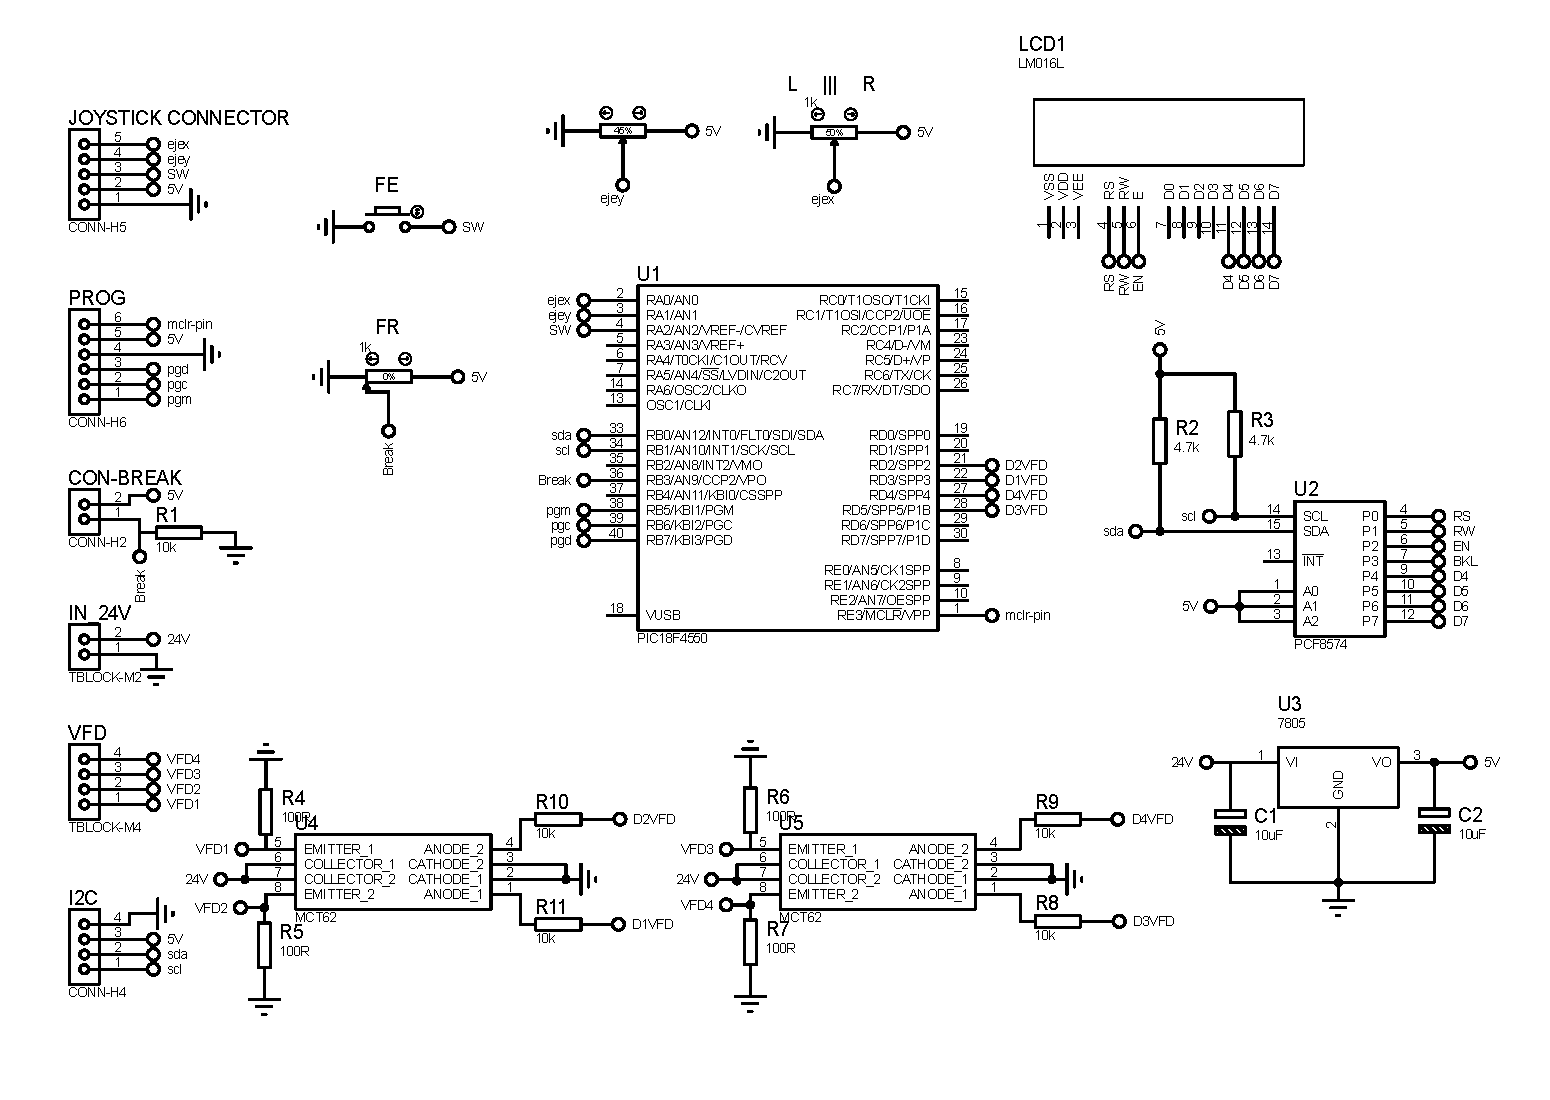
\includegraphics[width=1.0\textwidth]{Figs/circuito_electronico.eps}
\caption{Diagrama esquem�tico para tarjeta electr�nica dise�ada}\label{esquema}
\end{figure}		


Asimismo, la Fig. \ref{mandoboard} presenta el dise�o de la capa de componentes y de ruteado circuital para el montaje del circuito impreso (i.e. \emph{PCB}), al igual que la apariencia final de la tarjeta de mando electr�nico incorporada en el volante del veh�culo.\\
% ------------------------------------------------------------------------
\begin{figure}[htbp]
\centering
		\subfigure[Capa de componentes]{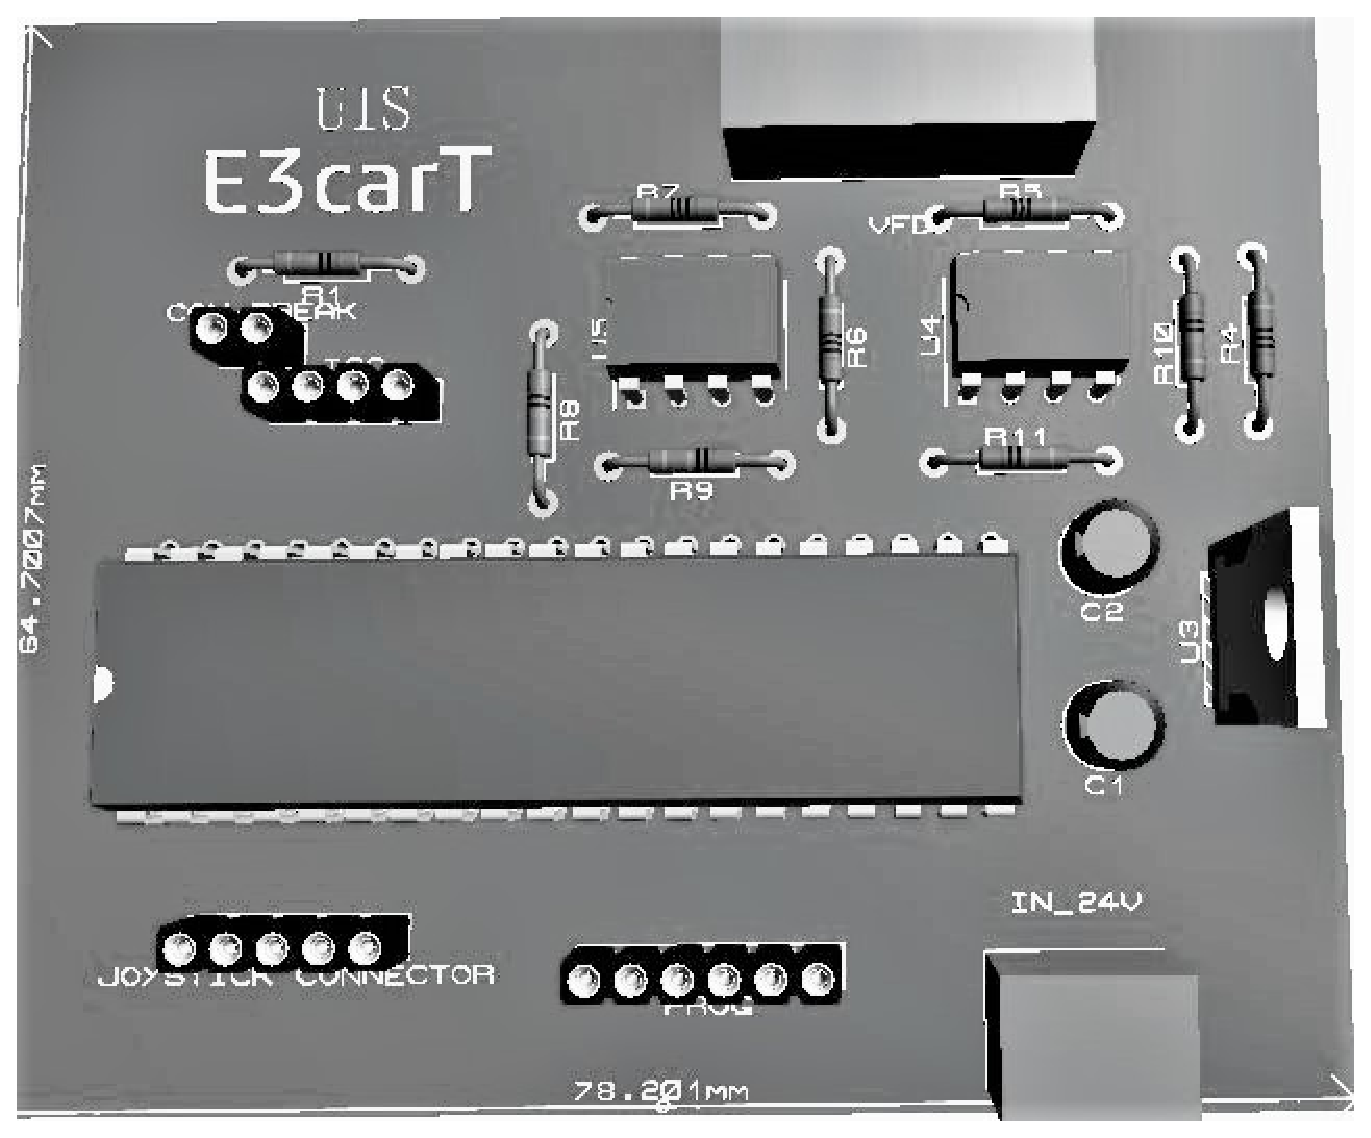
\includegraphics[width=0.45\textwidth]{Figs/pcb3d.eps}}
		\subfigure[Capa de ruteado]{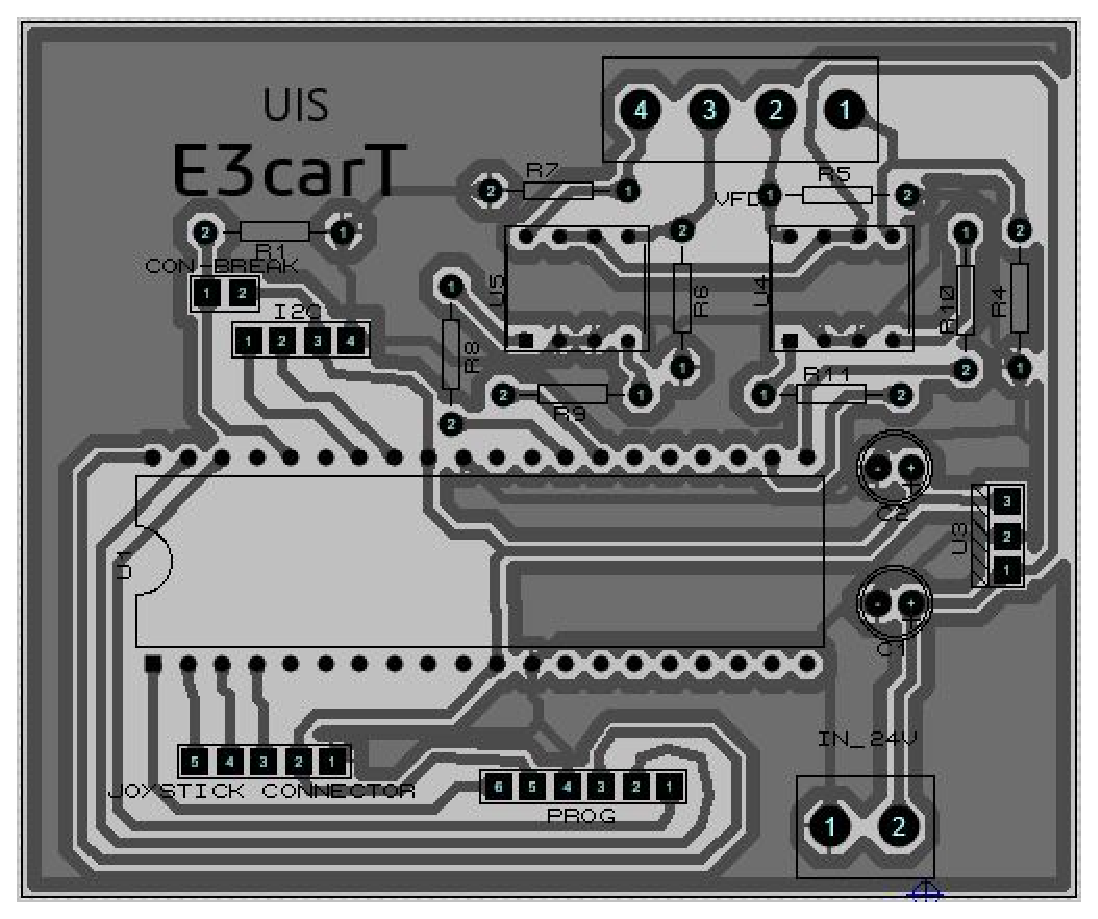
\includegraphics[width=0.45\textwidth]{Figs/PCB_gray.eps}}\\
		\subfigure[Apariencia final en volante]{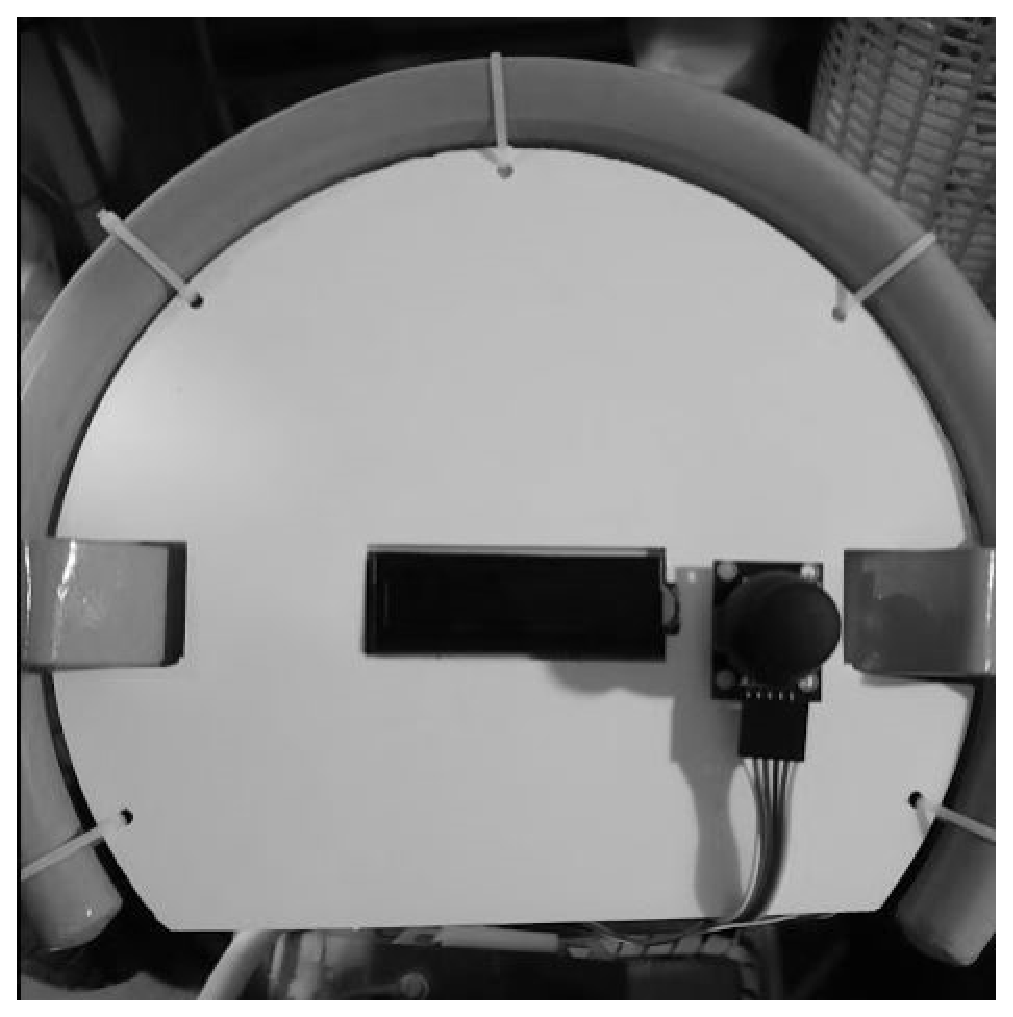
\includegraphics[width=0.45\textwidth]{Figs/volante_pcb.eps}}
		\caption{Dise�o de tarjeta de mando electr�nico.}\label{mandoboard}
\end{figure}
% ------------------------------------------------------------------------

Una vez dise�ada e implementada la unidad de mando electr�nico (hardware), es necesario realizar la implementaci�n del aut�mata correspondiente a la operaci�n deseada del veh�culo. Para ello se definen los estados operativos del sistema a partir de la m�quina de estados finita ilustrada en la Fig. \ref{fsm}.\\
% ------------------------------------------------------------------------
\begin{figure}[htbp]
\centering		
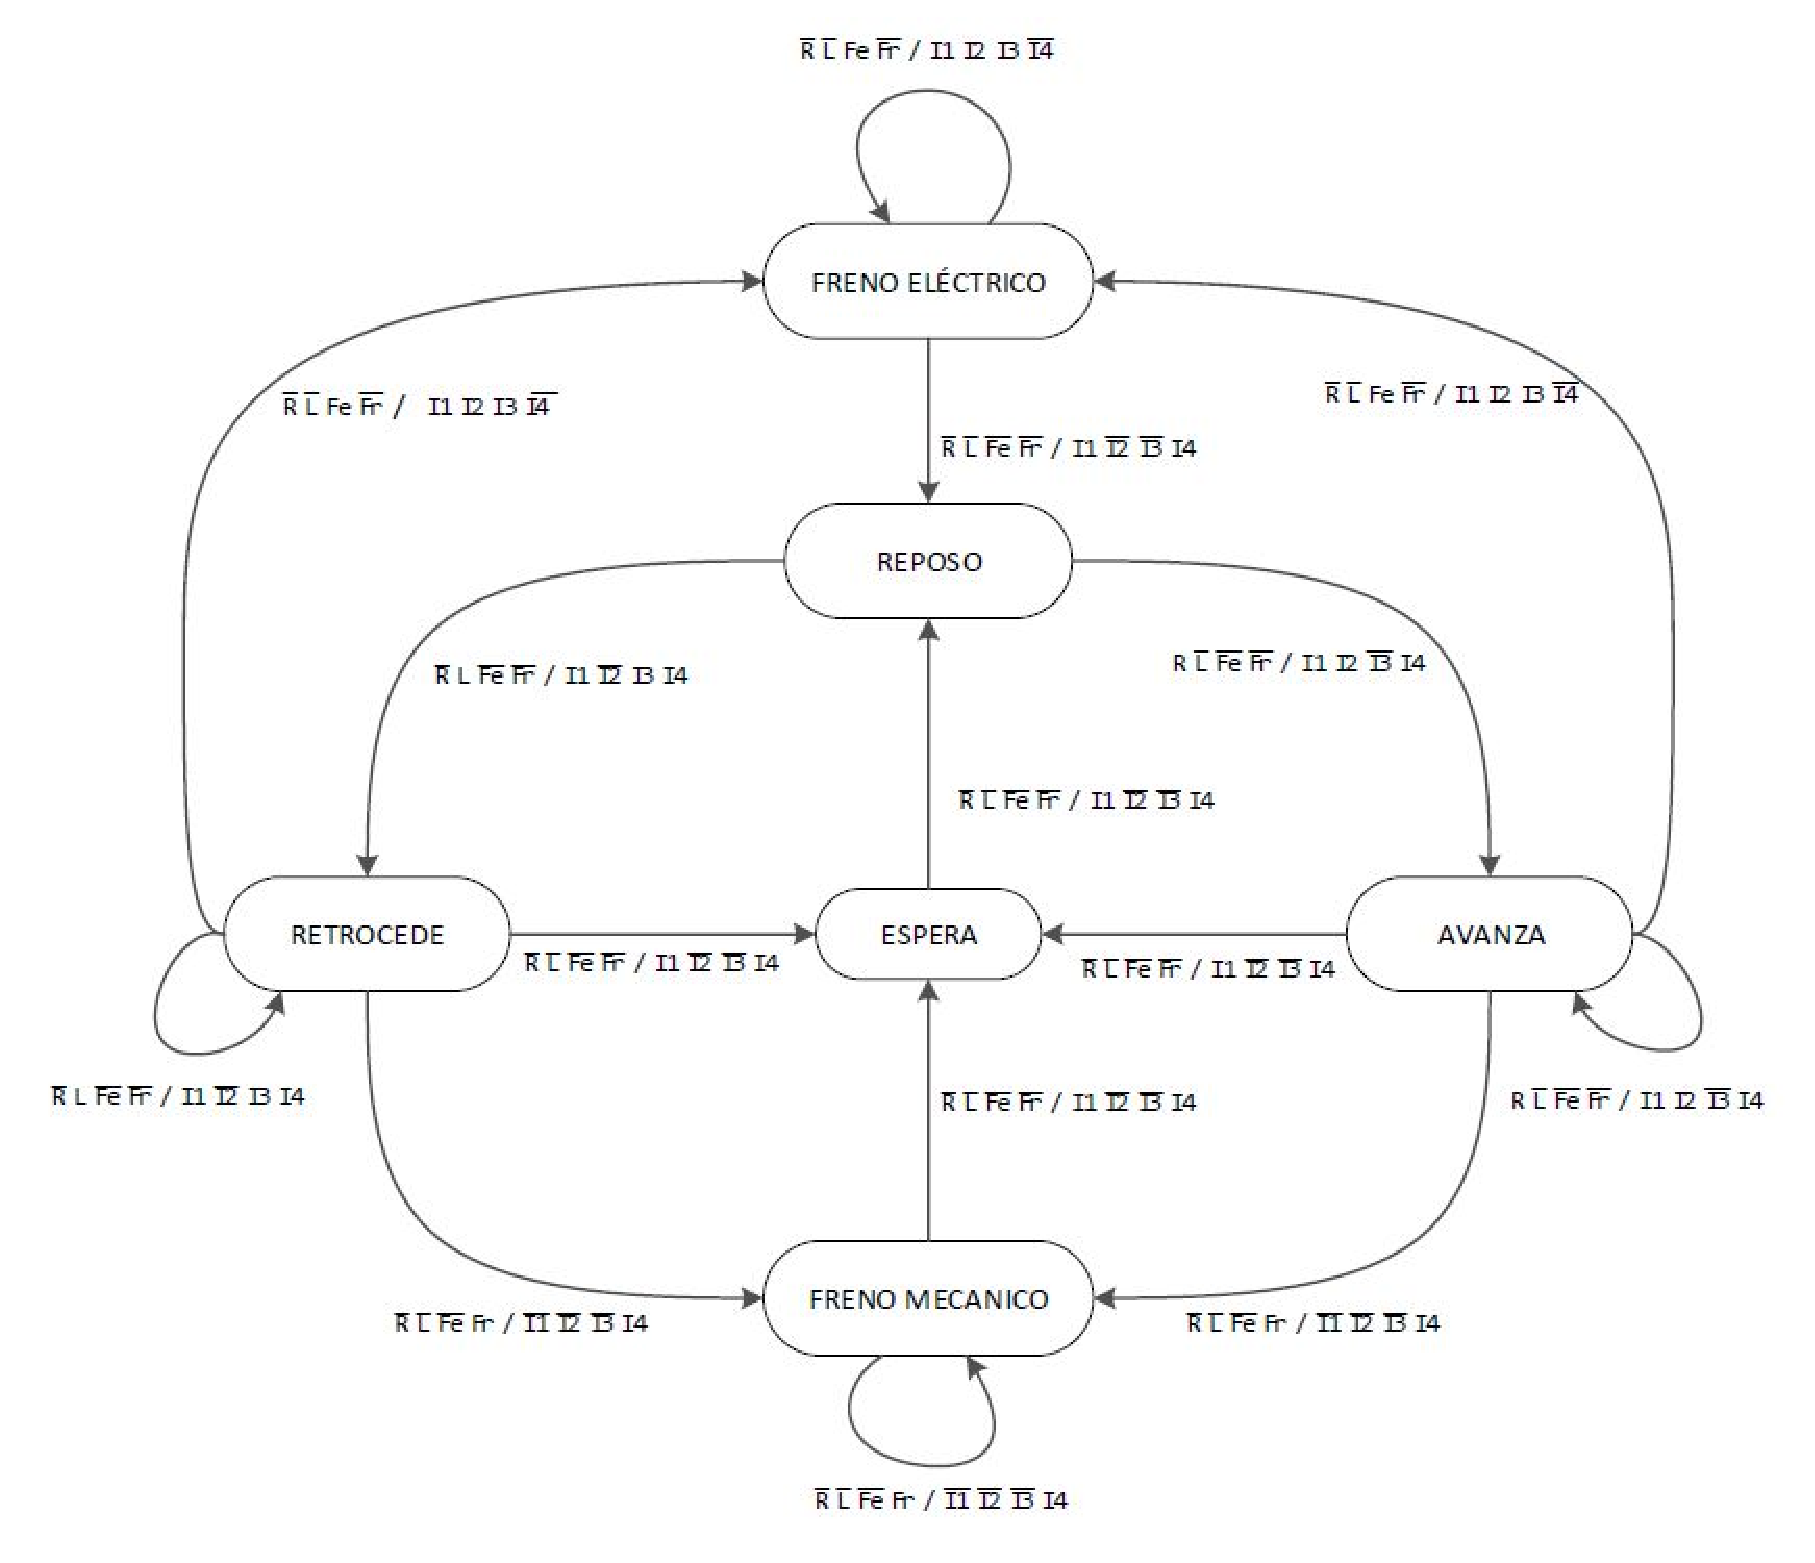
\includegraphics[width=1.0\textwidth]{Figs/fsm.eps}
\caption{M�quina de estados de operaci�n para comando electr�nico del veh�culo}\label{fsm}
\end{figure}
% ------------------------------------------------------------------------

A partir de ello, la operaci�n del motor se define empleando las entradas digitales del VFD (\emph{I1 I2 I3 I4}) considerando los siguientes comandos de acci�n:
% ------------------------------------------------------------------------
\begin{itemize}
\item[\emph{I1}:] Se configur� en modo \emph{ON/OFF1} a partir de la instrucci�n $P0701=1$. Un nivel de entrada alto activa la operaci�n del VFD, mientras que un nivel de entrada bajo activa un frenado el�ctrico tipo rampa con tiempo $P1121=10$ [s];
\item[\emph{I2}:] Se configur� en modo \emph{selector de frecuencia fija bit0} a partir de la instrucci�n $P0702=15$. Un nivel de entrada alto activa el giro del motor hacia la izquierda (i.e. \texttt{AVANZA}) a velocidad fija de $P1001=-60$ [Hz], incrementada desde el reposo por una rampa con tiempo $P1121=30$ [s];
\item[\emph{I3}:] Se configur� en modo \emph{selector de frecuencia fija bit1} a partir de la instrucci�n $P0703=16$. Un nivel de entrada alto activa el giro del motor hacia la derecha (i.e. \texttt{RETROCEDE}) a velocidad fija de $P1002=30$ [Hz], incrementada desde el reposo por una rampa con tiempo $P1120=10$ [s];
\item[\emph{I4}:] Se configur� en modo \emph{OFF2 - coast to standstill} a partir de la instrucci�n $P0704=3$. Un nivel de entrada bajo desactiva el VFD, permitiendo un frenado mec�nico en rodadura libre.
\end{itemize}
% ------------------------------------------------------------------------

El detalle de todas las instrucciones de configuraci�n para el VFD se encuentran detalladas en el manual proporcionado por el fabricante \cite{siemens2014}.

\newpage
\begin{center}
\textcolor[rgb]{0.98,0.00,0.00}{\textbf{HASTA AQU� VOY CON LA REVISI�N.....}}
\end{center}
\newpage

%% ------------------------------------------------------------------------
%\section{Cotizaciones y compra final}
%% ------------------------------------------------------------------------
%El d�a 22 de mayo de 2020 se realiz� la siguiente solicitud de gesti�n de compra de estos equipos v�a correo electr�nico, a trav�s del Ing. Juli�n Eduardo Blanco Cortez:\\
%% ------------------------------------------------------------------------
%\begin{itemize}
%\item Un (1) motor de inducci�n, tipo jaula de ardilla, de 2 HP, 1800 RPM, 60 Hz, 220/230 VAC, tipo NEMA C, con base del tipo "foot mounted". Marcas tentativas del producto: WEG, Siemens, ABB;
%\item Un (1) variador de frecuencia con salida para motor trif�sico (220/230) de 2 HP, con entrada de alimentaci�n monof�sica a 120 VAC / 60 Hz, que posea opciones de frenado del tipo: rampa, coast, injection. Marcas tentativas del producto: WEG, Rockwell Automation, SIEMENS, Danfoss;
%\item Un (1) inversor cargador, de 12 VDC a 120 VAC / 60 Hz, con potencia de 2 kW. Marcas tentativas del producto: Gen�rica;
%\item Cinco (5) ruedas neum�ticas de 14 pulgadas. Marcas tentativas: Roller;
%\item Una (1) bater�a recargable �cido-plomo de 12 V / 120 Ah, de ciclo profundo y peso no mayor a 40 kg. Marcas tentativas: Varta, NPP, Rolls. La imagen del elemento se adjunta al presente correo.
%\end{itemize}
%% ------------------------------------------------------------------------
%A la cual se adjuntaron las im�genes de la Fig. \ref{Elementos_cotizados}.\\
%
%% ------------------------------------------------------------------------
%\begin{figure}[htbp]
%\centering		
%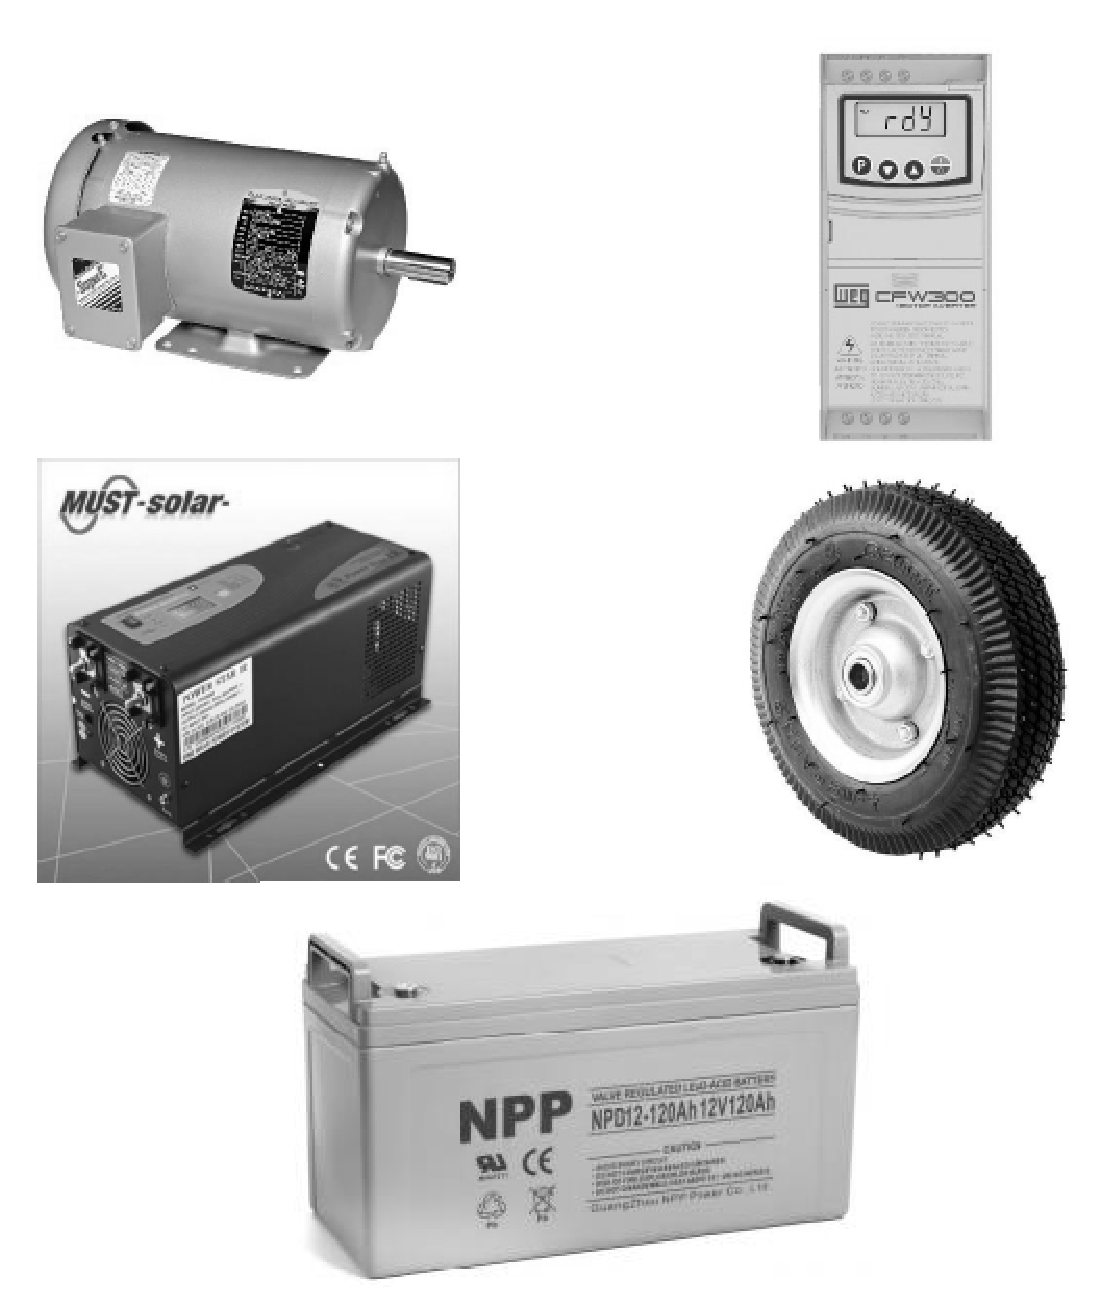
\includegraphics[width=0.5\textwidth]{Figs/Elementos-cotizados.eps}
%\caption[Elementos cotizados]{Im�genes adjuntas al correo en el que se envi� la cotizaci�n final a la Universidad.}
%\label{Elementos_cotizados}
%\end{figure}
%% ------------------------------------------------------------------------
%Se inici� un estudio de mercado con los proveedores reconocidos por la UIS y se les solicit� enviar la cotizaci�n de estos elementos, a la cual contestaron 5 proveedores: CASA HERMES LTDA., DYNAMO ELECTRONICS S.A.S, SUCONEL S.A., NARVAEZ INGENIER�A S.A.S., y SOLUCIONES INDUSTRIALES INTELIGENTES S.A.S. Estas se adjuntar�n como archivos separados.\\
%
%De estas se concluy�: la cotizaci�n de elementos realizada por CASA HERMES LTDA se present� como la m�s completa en cuanto al cumplimiento de las especificaciones t�cnicas solicitadas. Sin embargo, no fue la oferta m�s econ�mica, en parte por la cotizaci�n de un inversor solar con algoritmo integrado MPPT, innecesario para la aplicaci�n en cuesti�n. La cotizaci�n realizada por DYNAMO ELECTRONICS fue la m�s econ�mica. Sin embargo, incumpl�a las restricciones de peso requeridas para la bater�a (m�ximo 40 kg), adem�s de no precisar que el motor de inducci�n cumpla la norma NEMA tipo C, incumpliendo parcialmente las especificaciones requeridas. La cotizaci�n realizada por SOLUCIONES INDUSTRIALES INTELIGENTES fue excesivamente costosa comparada con las dem�s ofertas comerciales, lo cual la hizo inviable. La cotizaci�n enviada por SUCONEL fue incompleta, pues no cotizaron el inversor/cargador. Asimismo, cotizaron llantas para veh�culos convencionales que no correspond�an a los requerimientos solicitados. La cotizaci�n enviada por NARVAEZ INGENIER�A a pesar de incluir todos los elementos, s�lo present� informaci�n t�cnica del variador de frecuencia y del motor. El motor cotizado fue de categor�a B, lo cual incumpl�a el requerimiento solicitado (tipo NEMA C). De los dem�s elementos no se realiz� descripci�n diferente a la solicitada en el requerimiento inicial.\\
%
%Se pidi� entonces realizar la compra a CASA HERMES LTDA, y en caso de no ser posible, realizarla a DYNAMO ELECTROICS. Esta �ltima fue la opci�n escogida.
%  % Dimensionamiento y adecuaciones
%\input{Secs/T2(profesor)} % correccion realizadas por el profesor
% ------------------------------------------------------------------------
\bibliographystyle{amsplain}                                % Bibliograf�a
\bibliography{xbib}
% ------------------------------------------------------------------------
\end{document}                                          % Fin de documento
% ------------------------------------------------------------------------ 